\documentclass[pdftex,12pt,a4paper]{report}

% Document settings

\usepackage{fullpage}
\usepackage{cite}
\usepackage{datetime} 
\usepackage{geometry}
\usepackage[pdftex]{graphicx}
\usepackage{verbatim}
\usepackage{todonotes}
\usepackage{array}
\usepackage{capt-of}
\usepackage[parfill]{parskip}
\usepackage{underscore}
\usepackage{url}
\usepackage{listings}
\usepackage{fancyvrb}
\usepackage{enumitem}
\usepackage[toc,page]{appendix}


\usepackage{courier}
\lstset{
         basicstyle=\footnotesize\ttfamily, 
         numberstyle=\tiny,      
	language=Java,
}
\lstloadlanguages{
         Java
}

\makeatletter
\g@addto@macro\@verbatim\small
\makeatother

\geometry{verbose,lmargin=3cm,rmargin=3cm}

\newcommand{\HRule}{\rule{\linewidth}{0.5mm}}


\begin{document}

\begin{titlepage}
\begin{center}

% Upper part of the page. The '~' is needed because \\
% only works if a paragraph has started.

\includegraphics[width=0.4\textwidth]{figure/crest.png}~\\[1cm]

\textsc{\LARGE Imperial College London}\\[1.5cm]

\textsc{\Large Final year project}\\[0.5cm]

% Title
\HRule \\[0.4cm]
{ \huge \bfseries Computer Music Improvisation \\
A Grammatical Approach For Jazz}\\[0.4cm]

\HRule \\[1.5cm]

% Author and supervisor
\begin{minipage}{0.4\textwidth}
\begin{flushleft} \large
\emph{Author:}\\
Cliff \textsc{Sun} \\
chs09@ic.ac.uk
\end{flushleft}
\end{minipage}
\begin{minipage}{0.4\textwidth}
\begin{flushright} \large
\emph{Supervisor:} \\
Professor Murray 
\textsc{Shanahan}
\end{flushright}
\end{minipage}

\vfill

% Bottom of the page
{\large \today}

\end{center}
\end{titlepage}

\chapter*{Abstract}%
\addcontentsline{toc}{chapter}{\numberline{}Abstract}%
Improvisation is often seen as a human activity, especially in the domain of music. Genre's such as Jazz and Blues are heavily based on the performer improvising on a set form. Improvisation can be seen as a creative process and creativity is a phenomena that is often attributed to humans. We also know that in order to perform a creative activity such as music improvisation (and in addition composition) one must already have a grasp of the large set of rules and musical theory involved in order to do so successfully.

But creativity itself however is difficult to quantify and measure. In addition creativity is interpreted differently by different people. In this report, we introduce a program that aims to model and replicate creativity in the form of music improvisation using a computer. We aim to study and evaluate two aspects of creativity, one as part of the end-product and one as part of the process that produces the end-product.

We introduce a program built from the ground up using rule-based approaches, such as using a grammar and the rules of musical theory. With this we hope to be able to produce convincing melodies that can pass off as human generated/composed sounds. Using the program and the pieces it produces we can then evaluate how listeners interpret creativity and evaluate how our program exhibits creativity. We hope that by doing this it can help us understand the separation between `creativity' and rules that need to be learnt. In addition we hope that the tool/program produced can be useful in aiding performers by providing them with improvisational ideas to further stimulate their creative processes.

\chapter*{Acknowledgements}%
\addcontentsline{toc}{chapter}{\numberline{}Acknowledgements}%
I'd like to first of all thank my supervisor Murray Shanahan for proposing a novel and interesting project and in addition for guiding me throughout the process and providing me with useful tips and ideas. Secondly I'd like to thank my good friend Heen-Wah Wai, an accomplished musician who helped me understand jazz music theory better and who aided my project by providing me with some improvised jazz piano pieces for my survey. In addition I'd like to thank my mentor and friend Tim Wood who helped me in the early stages of my project, along with Simon Colton and Geraint Wiggins for their initial input at the beginning and Mike Cook for his advice on the evaluation of the project.

I'd also like to thank everyone else who has taken part in my blind test survey to compare jazz improvisation pieces, they have all provided me with the information and feedback I needed to be able to successfully evaluate my project.

Lastly I'd like to thank everyone (professionally related and non-professionally related) who has helped me not only in this project, but in the past four years of my undergraduate degree. This includes my family, my colleagues/course-mates and my friends. I owe my university experience to these people and it would not be the same without them.

\setcounter{tocdepth}{2} % Set the depth of toc indexing

\tableofcontents

\pagebreak

\renewcommand*\thesection{\arabic{section}}
 
\pagebreak

\chapter{Introduction}

\section{Overview}
Jazz and Blues music are relatively modern genres, but they have significant history and playing in these genres involve a wide understanding of musical theory. As a genre Jazz is extremely vast and is difficult to define, however improvisation is a key element in jazz and so as a genre it lends itself well to a project based on computational creativity.

There have been many different approaches for melody generation/improvisation in blues and jazz over the years and many of them have involved an analytical (mathematical/statistical) approach. We explore a more grammatical approach which uses an abstract musical grammar which will allow us to create well-defined structures and rhythms for jazz melodies. Additionally we introduce a supervised learning based approach which tries to embody a sense of evolution/progression in our program by updating grammar rule weightings based on user evaluation (as a fitness function/test input data). 

\paragraph{Improvisation vs Composition}
Music improvisation can be defined as the creative activity of immediate composition, or `Composition on the fly'. In the case of this project, both terms will be used interchangeably. However, the act of improvisation usually encompasses the playing itself, whereas composition can be seen as just composing notes for playing later. Our project is not designed to solve the playing aspect of improvisation, and as such it is better stated that our project composes jazz solo's in the style of jazz improvisation.

\section{Motivation \& Aims}
Many current and past approaches use analytical methods (i.e. mathematical and statistical methods), such methods try to capture and abstractly learn the creative process of improvisation from jazz pieces/examples, i.e. the rules and constraints for improvising in the same style as the example. If we imagine the natural process of learning and creating music as a flow chart then such analytical methods start from the end and they try to learn and infer the rest of the process abstractly. 

As a side note, many approaches also treat the pitch and the duration of a note as coupled objects. The pitch is a vertical aspect (i.e. pitch changes) and the rhythm of the piece is a horizontal aspect and as such they can be treated as independent for the most part.

Just like any activity, Jazz improvisation is governed by many `rules' (though it is important to recognise that they don't necessarily need to be followed all the time). In the case of actual notes/pitches, musical theory (specific and non specific to jazz) plays an important role for improvisation, telling us which notes we could use in a certain section in the piece (which scales are feasible with which chords). Musical theory is extremely complex especially when dealing with scales and harmonies (as we shall see later in Chapter 2). We know that in order to be able to do such an activity, one must learn and embody these rules. By capturing a subset of the comprehensive set of musical `rules' as a knowledge base for the program we can create a tool that can generate a wide variety of music that are also pleasant to listen to.

Additionally, on the subject of rhythmic ideas in jazz, one of the constraints that we explore in this project is the use of an abstract grammar to produce abstract tone sequences. Such an abstract grammar constraints the rhythmic sequence of our notes whilst also constraining the type of notes that we can use. We aimed to use such a grammar to form the basis of the music generation, whilst also aiming to produce a general solution which takes in a grammar specified by the user to generate jazz music with, thereby not limiting the possibilities of what can be generated.

Evaluation of our program is also difficult, usually such projects will produce an output of an artistic form (music/art/literature) and as such evaluation can be very subjective depending on the person. A simple way we can evaluate the output and result of such a project (in terms of music) would be to do a blind test (a Turing test) to compare a similar human composed piece of music to the output of the new program. We can score the program and its output based on whether the listener can or can not identify which piece of music was compose by a computer and which was composed by a human and which they preferred. In addition we will use some well known models such as Simon Colton's FACE descriptor \cite{coltonface2011} to try and evaluate the creativeness of our program. This will be explained more in the Evaluation section.


\section{Project Domain - Computational Creativity}
The project comes under the area of computational creativity, and it's immediate uses and contributions are fairly novel. One of the main challenges of computational creativity is to understand and replicate the creative processes of human beings in a computer. Of course this is extremely difficult to do (as we discuss below). However, though we may not know exactly how creativity works, the study of computational creativity can help us further understand better the behaviour of creativity in humans. According to Pease and Colton \cite{pease11}, there are 3 main motivations for studying computational creativity:

\begin{description}
  \item[Cognitive Science] to provide a computational perspective on human creativity, in order to help us understand it.
  \item[Engineering] to enable machines to be creative, in order to enhance our lives in some way.
  \item[Aiding Creative Individuals] to produce tools which enhance human creativity. 
\end{description}

Much work has been done in the field of generated visual art with tools and programs such as Simon Colton's Painting Fool \cite{website:paintingfool} and Harold Cohen's AARON \cite{website:aaron} both of which create original artistic images to a high standard.

\subsection{Understanding \& Interpreting Creativity}
It is very difficult to objectively defined creativity and to measure creativity in a quantitive way. First of all the definition of `creativity' is open to interpretation and as such, `creativity' is often referred to as a phenomena, and not a concrete process that can be observed in the human brain. For our purposes we have not tried to define creativity, nor have we tried to come up with some quantitive measure for the output of our program as this is out of scope of the project. As creativity is difficult to define, it is also difficult to recognise and explain as a separate process. As such, though it may seem that we haven't implemented an abstract concept of creativity in our program (i.e. a concrete creative process that is labelled as such), through embodying the musical theory in the program and using heuristics for note selection, we may have imparted an idea of creativeness into the program already. 

\section{Related Works}
Work on computer music improvisation dates back 20-30 years or so. One famous example of computer generated music in general is David Cope's EMI (Experiments in Music Intelligence) which produces music in the style of various composers (using existing works as input sources). In terms of computer improvisation for jazz and blues music, there have been numerous analytical (statistical and mathematical) approaches. One such approach based on machine learning techniques includes `Finding temporal structure in music: Blues improvisation with LSTM recurrent networks' By Eck and Schmidhuber (2002) \cite{eck02}. Belinda Thom's Band-out-of-a-Box (BoB) describes an interactive soloist which can improvise with another performer using unsupervised learning in `Unsupervised Learning and Interactive Jazz/Blues Improvisation' (2000) \cite{thom2000}. In addition Markov chains have been used to analyse and model jazz improvisation such as `Markov Chains as Tools for Jazz Improvisation Analysis' by Franz (1998) \cite{franz98} and `Improvising Jazz With Markov Chains' by Marom (1997) \cite{marom97}.

Other works regarding grammatical approaches for music improvisation include approaches based on string rewriting grammars (L-systems) in `Grammar Based Music Composition' by McCormack (1996) \cite{mccormack96}. In addition `A Grammatical Approach to Automatic Improvisation' by Keller and Madison \cite{keller07} introduces a formal grammar for music improvisation in which we will be basing our work on (see more below).

In addition and in relation to Keller's above mentioned paper \cite{keller07} we also note that work has also been done by Keller to learn jazz grammars from a corpus of jazz melodies. Learning Jazz Grammars by Gillick, Tang and Keller \cite{kellergillick09} uses a machine learning approach (combining clustering and markov chains) to learn abstract grammars which can be used to produce jazz melodies (similar to the system that \cite{keller07} produced). 


\section{Report Outline}
The rest of the report is laid out as follows:
\begin{description}
  \item[Chapter 2] provides some background on music theory and in particular some Jazz theory and ideas that are commonly used to improvise Jazz with.
  \item[Chapter 3] describes a simple approach without using a grammar to allow us to contrast the differences between grammatical and non-grammatical approaches
  \item[Chapter 4 \& 5] contains the main body of this report, it goes over the main grammatical approach that we have used, based on Keller's paper \cite{keller07} and also we describe a novel extension which allows the program to update the input grammar weightings using the user/listener as a fitness function/the evaluator.
  \item[Chapter 7] explains the evaluation process that we have gone through to measure the success and achievement of the project. This includes surveying users on comparing human composed jazz and computer composed jazz (from this project) and in addition we use some models/criteria for measuring the 'creativeness' of our final program.
\end{description}

\pagebreak

\chapter{Background - Musical Theory}

\section{Overview}
In this chapter we aim to provide some background on musical theory that is used in jazz and musical theory overall. The overall idea was to abstractly capture this information as a knowledge base for the program. We first start off by revising the concepts of chords and scales.

\section{Basic Music Theory}
\subsection{Scales}
A scale is a set of notes ordered by frequency/pitch that spans an octave. They can be played over multiple octaves in a repeating pattern and in addition played in ascending and descending order. A scale has a key associated with it, where the name of the key indicates the tonic (first note) and the tonality of the scale. For example the most basic scale is the C-major scale as seen in figure \ref{fig:cmajorscale}, which has 7 notes starting from tonic C: C,D,E,F,G,A,B and has a major tonality (bright when compared with minor which has a dark tone). The C-major scale is a Heptatonic (and Diatonic) scale which is the type of scale that is commonly associated with western music. Scale theory is quite complex however and won't be explored further. The basic concept of a scale is enough to understand the rest of the musical theory.

\begin{figure}[here]
  \centering
  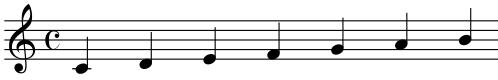
\includegraphics[scale=0.6]{figure/cmajorscale.png}
  \captionof{figure}{C Major scale}
  \label{fig:cmajorscale}
\end{figure}

\subsection{Chords}
A chord is a group of notes that are played together (at the same time) to give a fuller and more harmonious sound. They are often derived from scales, with the simplest chord being a triad, a set of three notes seperate by third intervals, i.e. 1, 3 and 5. Revisiting the C major scale, we see that the first, third and fifth of the scale is C, E and G. This when played together forms the C major triad as seen in figure \ref{fig:cmajortriad}. Often chords are played in the bass clef and form the accompaniment to the melody. 

It is important to note however that in jazz music, the third and the seventh note are the most important in a chord. These two scale degrees indicate the tonality of the chord (whether it be major, minor, dominant). A chord with a seventh scale degree is known as a seventh chord. These chords are used widely in Jazz as the sound of the chord is fairly destabilising, and thus indicating movement in the music. If we add a B flat to the C Major triad chord, we get a C Dominant Seventh chord as show in figure \ref{fig:cdominantseventh}. The dominant seventh chord is the most used seventh chord especially in classical music and jazz.

\begin{figure}[here]
  \centering
  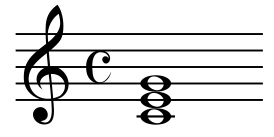
\includegraphics[scale=0.4]{figure/cmajortriad.png}
  \captionof{figure}{C Major Triad chord}
  \label{fig:cmajortriad}
\end{figure}

\begin{figure}[here]
  \centering
  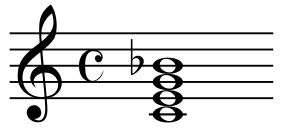
\includegraphics[scale=0.38]{figure/cdominantseventh.png}
  \captionof{figure}{C Dominant Seventh chord}
  \label{fig:cdominantseventh}
\end{figure}

As we shall see later, many different scales (and modes) can accompany a particular chord, as long as the chord can be derived from the scale itself.

\section{Blues Improvisation}
Blues is one of the most common genres that relies on performer improvisation. Performers of this genre tend to play a musical instrument (including voice) on top of an accompaniment with a well defined structure/form. The blues form itself is often defined by its 12 bar chord progression (commonly called 12 bar blues) which is essentially a standard harmonic chord progression of 12 bars in a standard 4/4 time signature. Table 1.1 below shows the chords for the general 12 bar blues form, with I7 referring to the harmonic seventh Tonic chord. Chord IV refers to the `dominant' chord (4th degree) and Chord V refers to the `dominant' chord (4th degree).

\begin{table}[here]
\centering
\newcolumntype{C}{>{\centering\arraybackslash}m{23pt}<{}}
\begin{tabular}{|*{12}{C|}}
  I & I or IV & I & I7 & IV & IV & I & I7 & V & V or IV & I & I or V
\end{tabular}
\caption{12 bar blues chord progressions}
\label{12 bar blues}
\end{table}


\begin{table}[here]
\centering
\newcolumntype{C}{>{\centering\arraybackslash}m{23pt}<{}}
\begin{tabular}{|*{12}{C|}}
  I & I & I & I & IV & IV & I & I & V & IV & I & I
\end{tabular}
\caption{12 bar blues simplified chord progression}
\label{12 bar blues}
\end{table}

Table 1.2 gives us one possible (and simple) chord progression for 12 bar blues in which we will basing our improvisation upon. 

\subsection{Blue Notes} What really gives the blues genre it's characteristics are the `blue notes'. These are notes which are played at a lower pitch (flatter) than that of the major scale (usually one semitone lower on piano). The notes which are `flattened' are the \textbf{third}, \textbf{fifth} and \textbf{seventh} notes of the major scale.
There are theoretical reasons for the introduction of `blue notes' which we won't go into detail here. But essentially these `blue notes' allow for moments of expression in blues melodies. 

\subsection{Blues and Pentatonic Scales}
Blues scales include the blue notes that we've mentioned above, these scales give the performer a set of notes to improvise with and gives the music the characteristic `blues' feel to it. Blues scales are generally based on the major/minor pentatonic scale. A pentatonic scale is a scale of five notes (compared to seven notes in regular major/minor scale) and is widely used in music across the world. The most common blues scale (and the one we are going to be basing our improvisations on) is the blues minor scale which is based on the minor pentatonic scale (see Figure \ref{fig:cminorpentatonicscale}) with a sharp 4th note (or a flat 5th note, both are equivalent). In Figure \ref{fig:cminorbluesscale} we can see the blues minor scale includes all the blue notes; E(3rd degree) flat, G(5th degree) flat and B(7th degree) flat \footnote{http://en.wikipedia.org/wiki/Jazz_scale\#Blues_scales, http://commons.wikimedia.org/wiki/File:C_minor_pentatonic_scale.png}.

\begin{figure}[here]
  \centering
  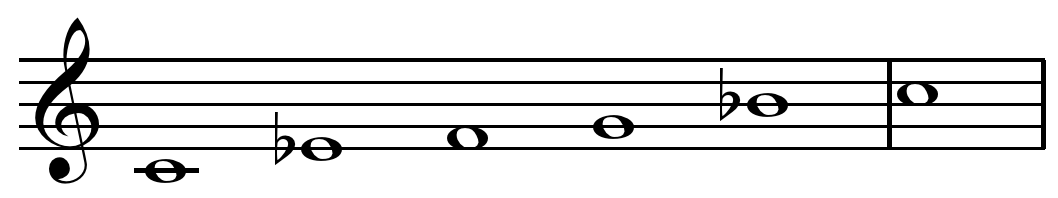
\includegraphics[scale=0.25]{figure/minorpentatonicscale.png}
  \captionof{figure}{C minor pentatonic scale}
  \label{fig:cminorpentatonicscale}
\end{figure}

\begin{figure}[here]
  \centering
  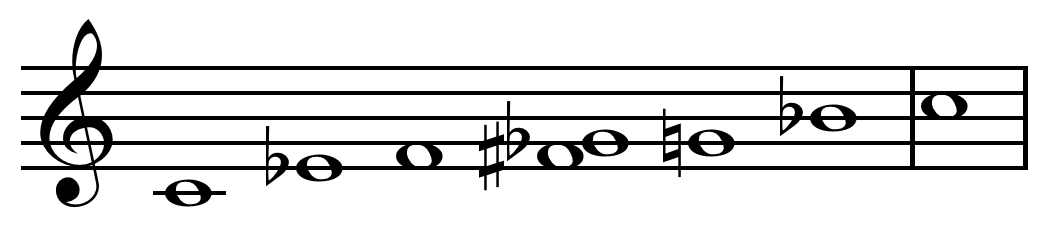
\includegraphics[scale=0.25]{figure/bluesminorhexatonicscale.png}
  \captionof{figure}{C minor blues (hexatonic) scale}
  \label{fig:cminorbluesscale}
\end{figure}

\section{Jazz Improvisation}

\subsection{Versus Blues}
Though it is common to use terms blues and jazz interchangeably, the reality is that they are very much different styles of music. However it is very difficult to categorise these two genres of music and much of the genre is overlapping. We'll refer to our music as fitting both jazz and blues during this report.

Blues itself has a very simplistic style, it relies on basic chord progressions (I IV V as we've seen above) which are repeated over and over again. By using one scale (pentatonic or minor blues scale) we can easily improvise a melody on top of the progression. In addition feeling and emotion is important in blues music and thus blues is based more on expression rather than technical ability. 

Jazz has many roots in blues music (in fact the blues form is ubiquitous in jazz music), the 12 bar progression is commonly used in Jazz music in addition to blue notes for expressive purposes. However Jazz itself is much more complex than blues and uses many more chords/scales, time signatures and melodic structures than blues. For example Jazz's rhythms tend to use syncopation (playing on the off beat) and swung notes i.e. playing two notes (which have the same duration) with different durations, where the first note has the longer duration and the second one the shorter. In addition Jazz chord theory itself is a very complicated as we shall see below.

\section{Basic Jazz Theory}
Jazz theory is extremely comprehensive and reflects in the complexity and the range of the music that belongs to this genre. It is useful to explain some musical theory that will not only help us understand improvisation, but music composition in general. Note that there is no right or wrong way to play music, there are many oddities in how the harmonic aspect of music works. Music theory (emphasis on the `theory') itself only aims to formalise (and standardise) a set of rules for music knowledge. In terms of jazz theory, books such as `The Jazz Piano Book' by Mark Levine provide a comprehensive learning guide to aid and teach jazz pianists the complex chord theory that jazz imposes. As it covers almost everything a beginner/intermediate jazz pianist needs to know to be able to improvise/play jazz, we will not go through everything from the book here. But we will highlight some of the more relevant ideas that we are using in our project.

\subsection{Chord Voicings}
Often a good way to start/learn simple jazz improvisation is to learn jazz chord voicings, these are essentially accompanying chords in the left hand which allows the pianist to use their right hand to play the melody and improvise. Chord extensions can be used to provide variations in the left hand voicings, for example adding the sixth, ninth and thirteenth scale note to the chord. Various progressions can be constructed using the large vocabulary of chord voicings, though many are based on the same underlying basic progression.

\subsection{Chord Substitution}
Chord substitutions are very common in Jazz, where a player/composer would use a chord in place of another related chord. Often it is just changing a note or two in the chord, but this small change often creates variety and interest and is what gives jazz music it's harmonic and melodic variety. The theory behind this is fairly complex and we won't be exploring this further, but the idea is that chord substitutions are possible and allow a richer variety in the music.

\subsection{Scale Theory - Playing Off the Chord}
As explained previously chord voicings allow us to have a varied left hand accompaniment which allows the right hand to improvise melodies. One simple way we can improvise melodies is to use scales that fit with the chord voicings. Indeed much of jazz is based on playing over the chords and being able to follow the chord changes itself. Certain scales fit different chords and thus it is up to the performer to choose the right scale to use to improvise a melody. Note that when we talk about scales here we do not mean in terms of sequence of notes, but rather the collection of notes that belong to the scale.

\subsubsection{Scales \& Modes}
For a simplified example, we can say that in the key of C major, the C major scale can be used over the II, V and I chord, i.e. Dm(7), G(7) and C. This is because for each chord, the 3rd and 7th note exists in the C major scale. We've discussed previously that the 3rd and 7th of a chord and scale indicates/identifies the tonality of the chord and scale. Thus it is reasonable to point out that scales with the same 3rd and 7th as a chord can be used to improvise on top of the chord.
If we look at it from another approach, then we can say that the chords used (and the tonality of the chords, i.e. major/minor/dominant) for the progression can be derived directly from the C major scale itself. To do this we must introduce an important piece of musical theory called modes. A mode is essentially a scale that can start from anywhere (not just the tonic C). There are 7 different modes in C major, each mode (scale) starting from a different note in the C major scale, below is an example of the 7 modes in C major and their corresponding names  \cite{jazzmusicmakers}.

\begin{figure}[here]
  \centering
  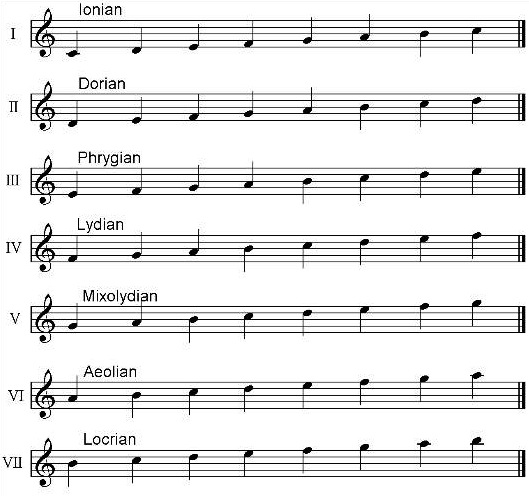
\includegraphics[scale=2.7]{figure/cmajormodes.jpg}
  \captionof{figure}{Modes for the C major scale}
  \label{fig:cmajormodes}
\end{figure}

If we look at the second (Dorian) mode we see that it starts from D and has an F natural and a C natural (3rd and 7th note respectively). This does not correspond to any D major/minor scale, which gives us the reason for having modes (allowing us to express and formalise different sequences of notes). If we take the 1st, 3rd and 7th of the Dorian mode, we get a D minor 7th chord (D, F, C), i.e. the II chord in our above progression. Similarly, if we take the fifth (Mixolydian) mode which starts from G, and we take the 1st, 3rd and 7th notes, we end up with a G dominant 7th chord (G, B, F). C major Ionian mode is trivial and thus we have our basic II-V-I progression derived from C major and it's modes. 
These modes also point out to us the avoid notes for each chord. The avoid note generally tends to be the 4th note, i.e. for the G7 chord, we use the fifth (Mixolydian) mode, where the C is the avoid note. This is because if you were to play a C on top of the G7 chord, it would sound dissonant. But avoid notes themselves can be used as passing notes where they don't have as much of a tonal impact in the music. As such, when we are in the key of C major and we have a dominant seventh chord in our left hand (G7), we can use the Mixolydian scale to improvise on top of the G7 chord. The above theory constitutes Major scale harmonies. It is also possible to `raise' the 4th note (augmented, annotated as +4) as an alternate to having the `avoid' note. For example we may use the first mode in C major (Ionian) and raise the 4th (F natural) to F sharp. We can see the effect of this in figure \ref{fig:clydian} taken from the Jazz Piano Book. In effect we have changed the key and as such the key happens to be G major. This means the new scale is in fact the C Lydian mode (in G major). However raising the 4th does not always in effect give us a new mode which corresponds to a different (major) key. Sometimes the new scale does not match any major key but rather is based on melodic minor scales. This brings us to Melodic Minor scale harmonies, however we won't go into this further, but it is important to realise the complexity of scales and scale theory not only for jazz, but for music in general.

\begin{figure}[here]
  \centering
  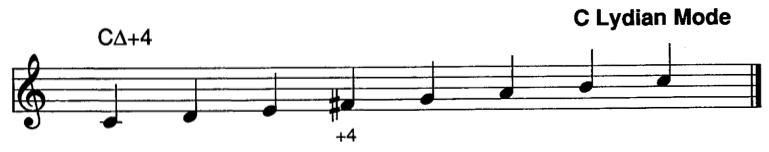
\includegraphics[scale=0.45]{figure/clydian.png}
  \captionof{figure}{C Lydian mode (in the key of G major)}
  \label{fig:clydian}
\end{figure}

Note in summary that it is important to think about the key that we are playing in, rather than the specific chord. We may end up using scales that are actually modes in alternative keys, which gives us musical variety in the improvisations.

\subsection{Chord - Scale System}
Following on from previously, the different scales and modes that we can use provide us with many alternative scales to use for improvisation over different jazz voicings. Different combinations of scales and chords have been used and developed over the years by the great jazz musicians, many of which had their own preferences for which types of scales to use for which voicings. This gives us a very diverse sound in jazz music and is what gives different players and musicians their own distinct style. 

\subsubsection{Dissonance - Avoid Notes} \label{avoidnotes}
One of the main concerns with the chord scale system is how it handles dissonance. Dissonance occurs when you have a combination of notes that sound harsh and unpleasant to the listener. In jazz music when using certain scales with chords, we may have some notes that we should 'avoid' as they sound harsh when played with the chord. Therefore they are known as `avoid' notes. However in reality we can use avoid notes as passing notes, though they are dissonant, they are fine as long as the dissonant note 'resolves' to a more harmonic note. Use of avoid notes and dissonance gives the music a 'jazzy' quality, for example in \ref{fig:avoidexample} the C\# is an avoid note in the C major scale but works fine as a passing note.

\begin{figure}[here]
  \centering
  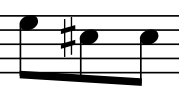
\includegraphics[scale=0.4]{figure/approachnormal.png}
  \captionof{figure}{Approach tone maintaining same direction}
  \label{fig:avoidexample}
\end{figure}


\begin{figure}[here]
  \centering
  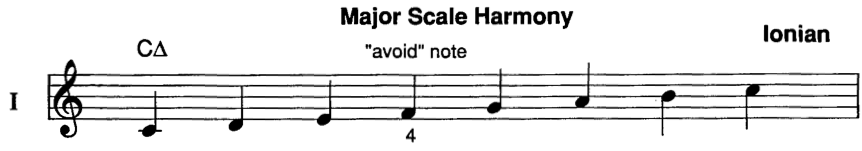
\includegraphics[scale=0.4]{figure/cionian.png}
  \captionof{figure}{C Ionian mode (in the key of C major)}
  \label{fig:cionian}
\end{figure}

Here we see that for a c ionian scale, with its accompanying chord, c major 7th chord ($\Delta$ indicates a major 7th chord), the F (the 4th/11th note) would be the avoid note.  In general for a major seventh chord (as we see above), the 4th note in the accompanying major scale is always the avoid note. But this is not necessarily the case for minor melodic scales, therefore it is not easy to determine which notes are 'avoid' notes. One way of defining avoid notes (which is not quite definitive in reality) is that the avoid notes tend to be the notes that are a half step (semitone) above the chord tones (1,3,5,7 intervals of the chord for example).

Overall it will be quite difficult to include all the scales and modes for major, minor and other harmonies. However our aim is to be able to represent the chord and scale theory as best as we can.

\section{Computer Improvisation For Blues/Jazz}

\subsection{Overview}
The idea behind jazz improvisation on the computer is that whilst jazz is essentially composition during performance (composition concurrent/on the fly), the composition is not completely done on the spot. Jazz musicians will practice many jazz licks, voicing's and scales before hand so that they can go into a performance with the required knowledge and practice needed to improvise jazz. Blues is also similar, blues musicians will practice pentatonic and minor blues scales whilst learning blues/jazz licks. Prior knowledge (knowledge of chord and scale theory) is a definite requirement in order be able to improvise blues/jazz at an advanced level.

\subsection{Difficulty/Complexity}
Blues and jazz music can range from something extremely simple such as playing the minor blues / pentatonic scale over a variation of the 12 bar blues progression, to complex theory involving left hand voicings, chord substitutions (tritone substitutions for example) and scale theory (and scale modes as we saw previously). Our aim is to be able to incorporate and encapsulate as much jazz theory as we can in the system that we are developing such that it can produce music with vast melodic and harmonic variations. Strictly speaking, the music that we generate may not strongly adhere to either a blues/jazz style (i.e. it may not easily identified with a jazz sub-genre or with a famous jazz musician) but is rather based on the ideas of blues and jazz improvisation. In addition the aim is to be able to provide a general solution that does not just produce a limited style and sound but rather be able to improvise a melody on any chord progression that we can give it. As a starting point, our goal is to generate/improvise jazz blues melodies on top of a 12 bar progression using a computer. Musical improvisation also covers improvisation/variations for the accompaniment as well. A grammar for comprehensive chord substitutions in improvising accompaniments in 12 bar blues/jazz is covered in Steedman's paper 'The Blues and the Abstract Truth: Music and Mental Models' \cite{steedman96}. However in this project our main focus is on melody generation.

Due to the project's time constraints and the complexity of jazz music, we are only aiming to be able to produce something that improvises jazz music to a beginner/intermediate level. The main challenge behind this project is the experimentation and uncertainty of using a grammatical approach to improvise music. Having a more realistic/achievable target (producing beginner's level jazz music) we have simplified the overall problem which allow us to concentrate on the technical aspect of the project.

\paragraph{Keys}
It is well known that the characteristic of music i.e. the listening experience is not based on the pitches of each note, but the pitch changes between each note. Thus a melody played in different keys will be recognisable to any listener familiar with the melody. For this reason we can simplify our problem further by working (melody generations/chord progressions) in the same key, the key of C. Transposition can be easily done by external tools and packages.

\pagebreak

\chapter{Initial Non-Grammatical Approach}

\section{Overview}
Before diving into a grammatical approach for blues melody improvisations, we decided to explore some simple ideas regarding probabilistic generation of notes in a sequence. Below are two simple approaches that we took. Note that we could easily classify these approaches with a simple grammar, however the point of introducing a grammar is so that we can defined structure and rhythm in our melodies, so for now we say that the first two simple approaches/implementations are not a 'grammatical' approach. 

\subsection{Simple Probabilistic Generation (with fixed duration)}
We decided to make a quick music improvisation tool which uses probabilities to pick the next note in the melody. We kept the duration constant (a quaver/eighth note) and kept the range within one octave. An example of the generation is shown below in Figure \ref{fig:randomgeneration}. We designed it so that the probability that we choose the next note has an inverse relation to the interval of the note itself. I.e. the probability is of choosing an adjacent note in the blues scale is highest, with the probability for choosing a note that is 2 notes apart lower. In addition we made it so that the probability that we choose a note so that sequence is going in the same direction is higher than choosing a note that changes the direction of the sequence. For example if we had an F (natural) followed by an F\#, the probability of choosing G is higher than choosing an F (natural) (both one note interval from F\#).

\begin{figure}[here]
  \centering
  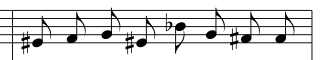
\includegraphics[scale=0.7]{figure/randomgeneration.png}
  \captionof{figure}{Probabilistic generation for a blues sequence}
  \label{fig:probabilisticgeneration}
\end{figure}

In the figure above we can see that a probabilistic random generation of notes with some constraints yields a fairly decent result. The notes are all part of the blues scale and so sound acceptable as a blues melody, however it lacks structure and rhythm as all the notes are of the same duration. 

\subsection{Probabilistic Generation With Mixed Durations}
To add some rhythm to the melody we decided that we could randomly choose duration lengths when we chose the next note. In our implementation we limited ourselves to semiquaver (16th), quaver (8th), and crotchet (quarter) notes. The idea was to introduce some style of rhythm to the music in the hopes of trying to make the melody fit into the blues criteria.

In Figure \ref{fig:randomgenerationwithdifferentdurations} we see an example of a bar that sounds fairly pleasing. We have an example of syncopation with the Eb quaver being played half a beat after the second beat. This sounds interesting and much more like blues music than in the previous example (in section 3.1). However not all bars generated look like this, some don't sound pleasing at all and some sound wrong rhythmically. As we are generating random durations, we are generating random rhythms and sequences and we may occasionally get a good melody, but a lot of the time we tend to get bad or awkward rhythms

\begin{figure}[here]
  \centering
  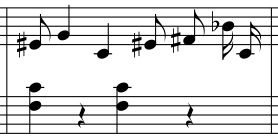
\includegraphics[scale=0.6]{figure/randomgenerationdifferentdurations.png}
  \captionof{figure}{Probabilistic generation with varying durations}
  \label{fig:probabilisticgenerationwithdifferentdurations}
\end{figure}

\subsection{Summary Of Non-Grammatical Approach}
The idea behind doing an initial non-grammatical probabilistic example is to show that first of all, rhythm is important in music. Different combinations of durations give us different rhythmic qualities, some of which sound wrong/awkward and some which sound pleasing. If we don't constrain the rhythmic aspects of the generated music then we end up with music that sounds random and unpleasing to the listener.
The other reason for doing the non-grammatical approach is that we can compare it to the results of using a grammar to generate music, thus allowing us to show the difference that using a grammar makes to the rhythmic aspects of the music.

\pagebreak

\chapter{Main Design - Grammatical Approach}

\section{Introduction}
In this project we propose a grammatical approach for generating blues melodies. Grammars have been used in other works in the field of computer music improvisation (see Chapter 1 - Related Works). We hope to be able to compare our approaches and results to mathematical and machine learning techniques for music improvisation/generation. 'Finding temporal structure in music: Blues improvisation with LSTM recurrent networks' By Eck and Schmidhuber (2002) \cite{eck02} is a more recent example of using LSTM networks to generate jazz bebop melodies. However there is a need for a training set and the result is affected by the quality of the training set. Using a grammar means that we don't need to encode a training set or input set and can directly influence our resulting sound.

\section{Grammars and Music}
Grammars by definition tell us how we structure words, phrases and sentences in an given natural language. From a linguists point of view a grammar is essentially a set of rules which needs to be learnt in order to speak a language. A simple grammar sentence structure would be $subject-verb-object$ which in turn is an important construct (most studied) in languages.
Therefore if we were to treat music as a language, where notes (i.e. pitch changes) are the words, phrases correspond to linguistic phrases and sequences of phrases form sentences, then we can expect that grammars can be used to describe the structure within music.The grammar can define the rhythmic aspects (i.e. structure) of the music, and as such a sequence of notes and it's rhythm can therefore give a melody it's own character and meaning, much like a sentence in natural language. However in music there are no semantic rules in terms of the melody, it is entirely up to the listener/player as to how they interpret it. This is where a grammar comes in, grammars are structural rules that govern the composition of 'sentences' (in the case of natural language) and such grammars are not concerned with the semantics of the sentence. Therefore a well-defined grammar for jazz music should be able to produce well-structured jazz melodies.

\subsection{Limitations of Grammars For Music} \label{grammarissues}
We acknowledge that there are some limitations for using grammars to generate music. A grammar has a finite search space and thus does not allow evolution of the improvisations of the program. Approaches that use inputs for training and analysing also suffer from the same problem too. However on the other hand we can come up with any grammar to use in the system which will in turn generate different pieces of music, much like other solutions that use machine learning / analytical approaches can generate different styles of music based on the given input training data.

\section{Adding a Grammar For Jazz}
The initial approaches are promising and give us a good foundation to build upon. If we randomly choose notes from a blues scale, they generally sound acceptable/good in terms of the pitch. However we have identified that some of the melodies/bars do not sound good rhythmically, i.e. they either don't sound good at all, or don't have the blues characteristics. We can see now that the rhythm of the notes is just as important as the pitch of the notes. 

In Keller and Madison's paper \cite{keller07}, a comprehensive grammar for blues is specified with excellent results. In particular a stochastic context-free grammar is used, where production rules of a context-free grammar are augmented with a probability/weighting. By using ideas from this approach we hope that we can create a more comprehensive grammar with more scope for variations. Note that the grammar should not recursive, as length is important in the generation of the terminal sequence. 

The terminal alphabet for the grammar is classified into different types of 'abstract tones'. A grammar can use these different types of tones to form a melodic sequence. The classification of different abstract tones is very much applicable to blues/jazz improvisation where knowledge of how to put these different types of tones together mean a better sounding melody is formed. In our previous non-grammatical examples, we use only notes from the blues scale. Though they sounded fine musically, using such a small set of notes means that the melody sounds flat and uninteresting for the most part and does not represent the widened Jazz musical genre. Additionally it is valid jazz to use notes that aren't part of the scale, they can be used as a 'passing note' for example and as such makes the melody sound more interesting and complete (see \ref{avoidnotes} on avoid notes). An article by Keller entitled 'How to Improvise Jazz Melodies' \cite{jazzkeller} talks about different methods for improvising blues/jazz melodies. The article provides many different methods and guidelines for improvising jazz/blues melodies. The above mentioned paper \cite{keller07} however only uses a few of these guidelines (albeit the most important ones). The classification of notes/tones are as follows:

\begin{description}
  \item[Chord Tones (\textit{C})] are tones (notes) which belong to the current chord we are improvising on top of.
  \item[Colour Tones (\textit{L})] are auxiliary tones for the current chord which sound correct musically when played with the current chord as an accompaniment. In particular, colour tones do not belong to the notes in the chord. 
  \item[Approach Tones (\textit{A})] are also notes which aren't in the chord (not the same as colour tones either) but they make good transitions to chord-tones or colour tones. These are also sometimes known as 'passing notes' where such a note can be placed between two chord/colours to make the melody seemed less disjointed. It is often bad practice however to place two approach tones next to each other.
  \item[Scale Tones (\textit{S})] are any notes that belong to the scale which works musically with the accompanying chord.
  \item[Other] tones which don't belong to any of the above. These may include a rest \textbf{(\textit{R})}, or a helpful tone \textbf{(\textit{H})} which is any of the above (C, L, A, S tones).
\end{description}

The issue we were concerned with before was whether we should deal with pitches of notes separately from the duration of the note. We have an option to create a grammar just for the rhythm of the melodic sequence. However randomly picking notes from the scale will not give us a result as good as the one in Keller and Madison 2007. The idea of chord, colour and approach tones provides us with a much better method of generating better sounding melodies.

\subsection{Context-Free Grammars}
The grammar described above is a context-free grammar. A grammar is considered context-free if the rules (production rules) of the grammar can be applied, i.e. the non-terminals can be written, without being dependant on the surrounding symbols. The majority of natural languages can be said to be based on context-free grammars. In addition we can say that the implementation of such a grammar for blues music is similar (and should be similar) to the implementation style of context-free grammars for random sentence generators. 

Context-free grammars are defined by the 4-tuple (V,$\Sigma$,R,S):

\begin{description}
  \item[V] - a finite set of \emph{variables}(non-terminal characters). Each variable essentially represents a different way to put together different families of notes and durations.
  \item[$\Sigma$]  - a finite set of \emph{terminals} which contain the actual content. In the case of our grammar, the terminals represent the type of tones/notes in the sequence.
  \item[R] - a set of production \emph{rules} in the form of A $\rightarrow$ b, where A is a variable $\in$V and b could be a sequence of variables and/or terminals.
  \item[S] - the starting variable/symbol used to represent the whole sentences where S$\in$V.
\end{description}


We start with starting variable S and expand the right hand side of the rule for S using other production rules. Expansion occurs by replacing variables in the sequence with the right hand side of the rule for that variable. We do this until the final result is a sequence of terminals only.

\subsubsection{Stochastic Context-Free Grammar}
The grammar that is defined in Keller's paper \cite{keller07} is a context-free grammar with probabilities, a stochastic/probabilistic context-free grammar. Each production rule has a probability associated with it which determines the likelihood of which production rule to use (if there are more than 1 with the same variable on the left hand side).

\section{Abstract Tone Grammar For Jazz}
We aim to implement the grammar described in the paper by Keller \cite{keller07} as a basis for jazz improvisations. The grammar itself is essentially a set of production rules which represent different rhythmic phrases with families of tones and their duration as the terminals. At the top level, we have the production rules P(n) $\rightarrow$ ... where n is the length of the melody generated in quarter/crotchet beats and n $\in$ 1..N:

\begin{verbatim}


P(0) -> empty [1]
P(1) -> Q1 [1] 
P(2) -> Q2 [1] 
P(3) -> Q2 Q1 [1] 
P(n) -> Q1 P(n−1)  [ .4 ]
P(n) -> Q2 P(n−2)  [ .4 ] 
P(n) -> Q4 P(n−4)  [ .2 ]

\end{verbatim}

A P variable takes in argument n, which limits the generation of the melody to fit n beats. We could also have a recursive grammar which expands until it reaches a set limit, but we may end up truncating a phrase which is not preferred. The values in the square brackets denote the weights for choosing a particular rule. It is worth noting that for the rules above, the weights are the same as probabilities (they add up to 1, so for P(n):  0.4+0.4+0.2 = 1), however it is not a requirement. The weights will will be normalised so that the actual probabilities are worked out.

The rest of the rules are taken from the aforementioned paper. We have rewritten the names of variables so that the numbers which follow a letter (i.e. Q4, V1, N/2 etc) denote the length of the notes generated (in quarter/crotchet beats). For example all the terminal sequences that can be generated from variable Q4 will have a total length of 4 crotchet beats. In addition, the number of beats that V/2 produces is half a beat (and also any other variable with /2). The specification of the grammar in Keller's paper \cite{keller07} is slightly inconsistent in the variable naming convention and can cause confusion. Therefore the rules (with new renamed variables) are as follows:

\begin{verbatim}

Q4 -> Q2 V1 V1  [0.52]
Q4 -> V/2 N1 N1 N1 V/2  [0.01]
Q4 -> V1 Q2 V1  [0.47]

Q2 -> N2  [0.06]
Q2 -> V1 V1  [0.6]
Q2 -> V/2 N1 V/2  [0.12]
Q2 -> H3/2 N/2  [0.16]
Q2 -> ({3} H1 H1 H1)  [0.06]

Q1 -> C1  [1]

V1 -> N1  [0.22]
V1 -> V/2 V/2  [0.72]
V1 -> ({3} H/2 H/2 H/2)  [0.05]
V1 -> ({3} H/2 H/2 A/2)  [0.01]

V/2 -> N/2  [0.99]
V/2 -> H/4 A/4  [0.01]

N2 -> C2  [1]

N1 -> C1  [0.5]
N1 -> L1  [0.2]
N1 -> S1  [0.5]
N1 -> A1  [0.01]
N1 -> R1  [0.25]
N/2 -> C/2  [0.4]
N/2 -> L/2  [0.2]
N/2 -> S/2  [0.4]
N/2 -> A/2  [0.01]
N/2 -> R/2  [0.1]

\end{verbatim}

In the N-variables, C, L, S, A and R are terminals in the terminal alphabet. They are shorthand for the families of tones that we've described at the beginning of the section. The grammar itself contains 4 distinct levels / types of variables:

\begin{description}
  \item[N-variables] - e.g. N2, N1 and N/2. These variables are at the bottom of the tree and their rule is always rewritten as a single terminal with the same length as the variable (see above).
  \item[V-variables]  - e.g. V1 and V/2. These are intermediate variables that describe small rhythmic sections. They allow the specification of different ways of making up a certain number of beats. For example we could add rules for V1 to represent more possible phrases, such as [V1 $\rightarrow$ H/4 N/2 H/4] if we wanted to add more variety to the music. They use the N-variables above to construct the sections. Note that the H-variable is a terminal which represents a \textbf{helpful} tone and refers to any of the Chord (\textit{C}), Colour (\textit{L}) and Approach (\textit{A}) tones.
  \item[Q-variables] - e.g. Q4, Q2, Q1. These are top level variables which essentially combine smaller sections/phrases to produce the larger sections. 
  \item[P-variable] - e.g P(n), the starting variable (as seen previously).
\end{description}

Again each rule has a probability associated with it and the above probabilities are taken from the above mentioned paper. The probabilities themselves play a large role in how the resulting melody sounds and at the moment can only be adjusted by the user.

Each unique derivation for each duration we generate for (the n in the P(n) starting variable) has its own unique parse tree. Figure \ref{fig:Q2parsetree} shows a partial parse tree just for Q2, which is already fairly comprehensive. We can see that the overall probability for generating a terminal sequence \emph{C1 C1} or \emph{C1 S1} from Q2 is $0.6*0.22*0.22*0.34*0.34= 0.00336$. It is worth noting that many more melodies can be created with one particular terminal sequence, which we will discuss below.

The implementation of the above grammar will give the same results as in Keller's paper \cite{keller07}, indeed changes and enhancements may be made along the way to try and improve the result. 
It would also be better if we could allow users to adjust the grammar themselves to produce different melodies, for example a more complex grammar would perhaps produce a more complex melody. 

\begin{figure}[here]
  \centering
  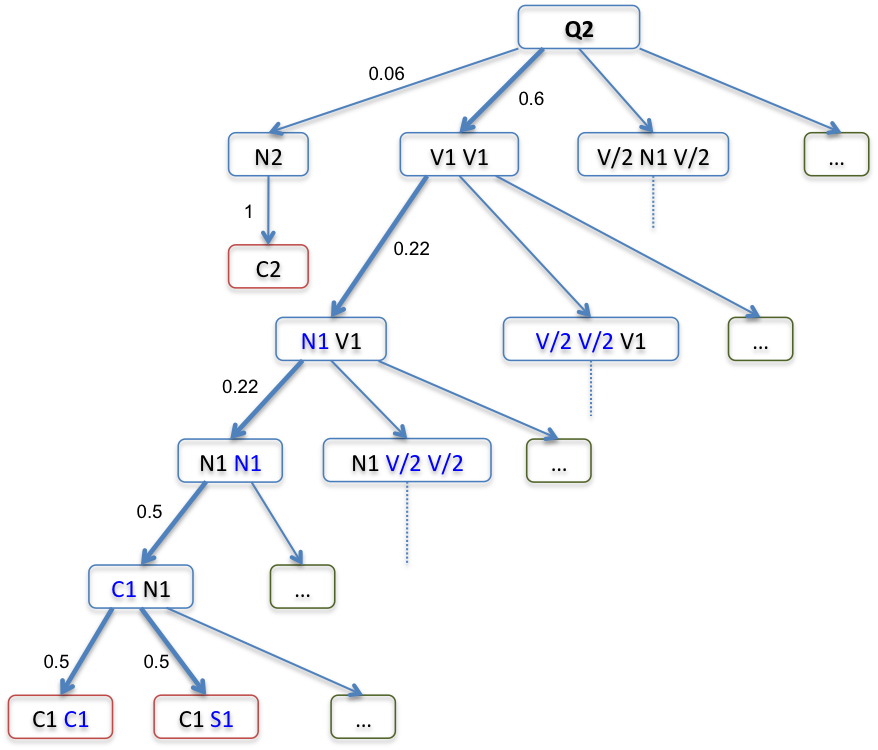
\includegraphics[scale=0.8]{figure/Q2parsetree.png}
  \captionof{figure}{Parse tree for Q2}
  \label{fig:Q2parsetree}
\end{figure}

\section{Terminal Sequences to Melodic Sequences} \label{terminalsequences}
As we've discussed previously, the grammar above generates a terminal sequence of types of tones and durations. Additional work needs to be done in order to produce a sequence of actual musical notes. An example terminal sequence that may be generated for P(4) $\rightarrow$ Q2 Q2 may be:

\begin{verbatim}
C/2 L1 H/4 A/4 H3/2 S/2
\end{verbatim}

We could generate many melodic sequences from the terminal sequence alone. However we would prefer to generate better sound melodies if possible. To do this we would have to introduce constraints when choosing actual musical notes from the families of tones, otherwise we may end up with a melody that sounds as random as our non-grammatical attempts. To do this we refer to Keller's article 'How to Improvise Jazz Melodies' \cite{jazzkeller}. Here are some possible ways we can constrain the selection of notes to ensure a better sounding melody:

\begin{description}
  \item[Know scales that go off the chords] scale here refers to a set of notes, rather than a sequence. If we know what scale works for the current chord, then it can help constrain the choice of tones so that the melody is closer to the scale.
  \item[Intervals between notes] smaller intervals often sound more pleasing than large intervals, however it is good to have both. If our intervals are too big then the melody will sound quite discordant (i.e. it will sound quite jumpy and erratic). However alternatively 'skipping' notes can sound good if combined with a direction change (see below) and can give a zig-zagged effect.
  \item[Change direction] if we have a sequence of small intervals (scale-like sequence) we may want to change direction at some point to provide variety and make the melody sound more interesting. We don't want to do this too often however as it may sound disorientating.
  \item[Use of enclosures] similar to direction changes, we can approach a note from both sides alternatively. This involves making sure intervals get smaller and also direction changes occur. Enclosures work better if the target tone is a chord tone.
\end{description}

By implementing these musical features, we can avoid awkward note combinations and optimise the melodic sequence from the terminal sequence. We will explore how to do this in the next section.


\section{Heuristics \& Methods For Note Selection}
There are different ways we could select the final note sequence from the abstract tone sequence. However we are not trying to find the 'optimal' solution as in reality there is no optimal solution when it comes to music. We can only hope that by following some guidelines and rules (from \ref{terminalsequences}) we may be able to generate better sounding melodies. We also have to be careful to make sure that our rules are not too fine grained so that it limits the variety of what we can generate. Variety is important for music and it allows for a range of musical expression.

Jazz improvisation is similar to any other creative activity, in that experience accounts for much of the performance. We explore whether it is possible to encapsulate such experiences as heuristics to generate the final jazz melodies. The idea of using a heuristic is that we can capture the current knowledge and experience associated with basic musical composition (and note selection) and use that to generate the actual musical notes. 

\subsection{Initial Steps}
Previously we mentioned that two approach tones next to each other may not sound good (due to a high chance of there being dissonance). So the first step is to make sure that if we have an Approach tone followed by another Approach tone, we need to convert the second Approach Tone into a different tone (default is Chord tone).
The abstract grammar essentially restricts our note selections by giving us a terminal sentence consisting of abstract tones. The tones tell us which notes will work at this point in the sequence/phrase. Of course there is still a lot that we could do to determine which notes are picked and as we've mentioned previously, many melodic sequences could be generated from the terminal sequence. 

\subsection{Globals}
We intend to have some global limits for note selection for which all algorithms can use. This is set as a properties file which can be read into the program. Currently we have an interval limit, which says how many semitones apart should the next note be within. In addition we also don't want to constrain the interval limit too much, sometimes having a large jump (octave changes for example) creates interest and variation, so we also set a probability that we select a note which has an interval from the previous note which is bigger than the interval limit. Finally we also set a maximum interval limit, such that no intervals between two notes can be bigger than this number. The values assigned below are gained from experimentation and based on existing experience and knowledge. An example of what our properties file would look like is here:

\begin{verbatim}
intervalLimit = 5
intervalLimitProb = 0.95
maxIntervalLimit = 9
\end{verbatim}

\subsection{Simple Heuristic}
We initially came up with a simple heuristic in which the next note depends on the note that immediately precedes it. This simple approach of course does not take in account for many of the things we discussed in \ref{terminalsequences}. Most importantly, approach tones are not really approach tones as they are only dependant on the note before it, when they should be dependant on the note after it.
The algorithm is quite simple:

\begin{verbatim}

function convertTonesToNotes(listOfTones)
  listOfFinalNotes = []
  previousNote = null
  for tone in listOfTones
    listOfNotes = getAvailableNotes(tone)
    if previousNote != null then
      listOfPotentialNotes = []
      for each note in listOfNotes
        rand = random number
        if rand > intervalLimitProb then
          if interval(note, previous note) <= maxIntervalLimit then
            add note to listOfPotentialNotes
          else
            nothing
        else
          if interval(note, previous note) <= intervalLimit then
            add note to listOfPotentialNotes
      add random note from listOfPotentialNotes to listOfFinalNotes
    else
      add random note from listOfNotes to listOfFinalNotes
  return listOfFinalNotes

\end{verbatim}

The idea behind it is simple, we take each tone from the list of abstract tones (starting from the beginning) and we get a list of suitable notes that can use. Initially we can randomly choose from this list. For the next tone we again get the list of suitable notes that we can use and again randomly pick one note as long as it satisfies the global interval constraints.

\subsubsection{Approach Tone issues}
The problem with the simple heuristic is that approach tones do not serve their intended purpose. They should be notes that 'approach' (i.e. come before) the next note, such that the approach note should be a note that is chromatically above or below the next note (i.e. one semitone away). Figures \ref{fig:lookbehindnoteselector} and \ref{fig:lookbehindnoteselector2} illustrate the problem. The F sharp in figure \ref{fig:lookbehindnoteselector} is the approach note selected based on the previous note F. However when this is played, it sounds awkward as the F sharp is not being immediately resolved and instead jumping down to a D afterwards. In figure \ref{fig:lookbehindnoteselector2} the D sharp does not sound as bad as the jump from D sharp to F isn't large and it continues in the same direction. Though these melodies are still fairly harmonious, the simple heuristic method doesn't handle approach tones as the grammar intends.

\begin{figure}[here]
  \centering
  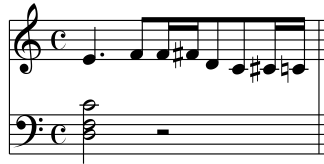
\includegraphics[scale=0.6]{figure/lookbehindnoteselector.png}
  \captionof{figure}{Example Bar using the Simple Heuristic 1}
  \label{fig:lookbehindnoteselector}
\end{figure}

\begin{figure}[here]
  \centering
  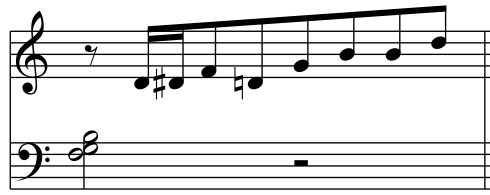
\includegraphics[scale=0.5]{figure/lookbehindnoteselector2.png}
  \captionof{figure}{Example Bar using the Simple Heuristic 2}
  \label{fig:lookbehindnoteselector2}
\end{figure}

\subsection{Better Heuristic}
It would therefore serve us better if we choose all the notes apart from the approach tones first and then choose the approach tones last. The idea behind this is that though we may be playing notes that are not on the scale (and may clash usually), they serve well as 'passing' notes such that after this note is played, it must be 'resolved' to a note that harmonically belongs to the accompanying chord. 

\begin{verbatim}


noteList = selectAllNotesApartFromApproachTones(listOfTones)

for tone in listOfTones
  if tone is an Approach Tone then
    nextNote = select next note in noteList
    prevNote = select previous note in noteList
    if prevNote is below nextNote then
      approachNote = semitone below nextNote (given probability p)
                or semitone above nextNote (given probability p-1)
    else
      approachNote = semitone above nextNote (given probability p)
                or semitone below nextNote (given probability p-1)
    add approachNote to noteList

return noteList

\end{verbatim}

We see that the algorithm above chooses the approach note based on the previous note additionally. Using different approach notes (above or below the next note) changes the expression of the melody as seen in figure \ref{fig:approachnormal} and figure \ref{fig:approachenvelope}. The user may want to set adjustable probability p in order to generate more of one type. Such a value of p can be gained experimentally, or inferred from an input training set (supervised learning).

\begin{figure}[h]
  \centering
  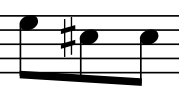
\includegraphics[scale=0.4]{figure/approachnormal.png}
  \captionof{figure}{Approach tone maintaining same direction}
  \label{fig:approachnormal}
\end{figure}

\begin{figure}[h]
  \centering
  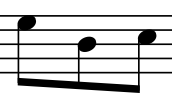
\includegraphics[scale=0.4]{figure/approachenclosure.png}
  \captionof{figure}{Approach tone forming an enclosure}
  \label{fig:approachenclosure}
\end{figure}

\subsubsection{Selection of Other Tones}
How would be go about selecting the other tones initially (i.e. how do we define $selectAllNotesApartFromApproachTones()$)? To do this we need to analyse and break down the act of simple jazz improvisation. We know that Chord Tones will have notes which are consonant (they work with and sound stable) the chord. As such, we know that melodies need to resolve to Chord Tones at certain points to reinforce the scale used on top of the chord. Keller's guide to jazz improvisation, \cite{jazzkeller}, mentions this idea and it is a good place to start.

One idea would be to generate Chord Tones first, and then generate 'Other' tones (Scale/Colour) Tones based on the Chord Tones:

\begin{verbatim}


function selectAllNotesApartFromApproachTones(listOfTones)
  listOfChordNotes = []
  chordMapping = <ChordTone, OtherTones[]>
  previousNote = null
  for tone in listOfTones:
    if tone is a Chord Tone then
      chordNote = chooseAppropriateChordNote()
      add chordNote to listOfChordNotes 
          in appropriate index
  for tone in listOfTones:
    if tone is a Colour or Scale Tone then
      if there are Chord Notes in the listOfChordNotes then
        assign tone to the closest Chord Note after the tone
        add to chordMapping
      else
        assign tone to the Tonic of the scale
  listOfFinalNotes = selectOtherTones(listOfTones, 
                                      listOfChordNotes, 
                                      chordMapping)
  return listOfFinalNotes


function selectOtherTones(listOfTones, listOfChordNotes, 
                                       chordMapping)
  listOfFinalNotes = listOfChordNotes
  for chordNote in listOfChordNotes
    otherTones[] = get otherTones for chordNote from chordMapping
    for tone in otherTones
      note = chooseAppropriateNoteForTone(tone)
      add note to listOfFinalNotes in appropriate index
  return listOfFinalNotes

\end{verbatim}

There can be numerous ways we can choose the appropriate notes ($chooseAppropriateChordNote()$ and $chooseAppropriateNoteForTone()$). The simplest way is to randomly choose the Chord note and then randomly choose the corresponding Colour and Scale notes (whilst imposing interval limits like in the Simple Heuristic). Of course randomness gives us greater variety in the generation of music but is not controlled and doesn't tell us why it chose to pick such notes. There is a possibility to explore better options for selecting Chord, Colour and Scale notes as further work. 

Figures \ref{fig:lookaheadapproach1} and \ref{fig:lookaheadapproach2} show us the correct way of using the approach tones as specified by Keller's paper \cite{keller07}. In figure \ref{fig:lookaheadapproach2} the last 3 triplet'd notes form a small chromatic run. The heuristic uses a probability to determine which type of phrases are generated more often (can be set by user).

%\vspace*{5\baselineskip}


\begin{figure}[h]
  \centering
  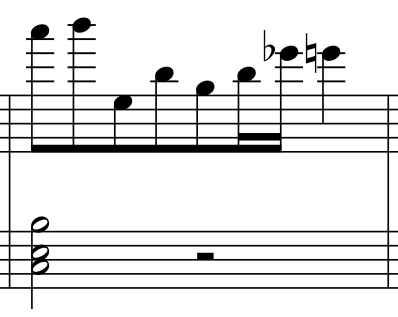
\includegraphics[scale=0.33]{figure/lookaheadapproach1.png}
  \captionof{figure}{E flat here is the approach note to E natural}
  \label{fig:lookaheadapproach1}
\end{figure}

\begin{figure}[h]
  \centering
  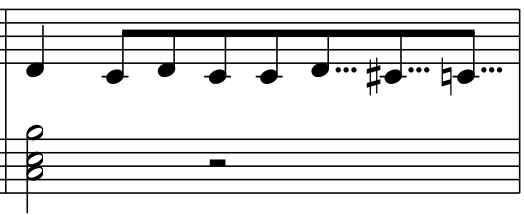
\includegraphics[scale=0.35]{figure/lookaheadapproach2.png}
  \captionof{figure}{Chromatic run has formed with C sharp being the approach note to C natural}
  \label{fig:lookaheadapproach2}
\end{figure}


\subsection{Probabilities as Decision Points} \label{decisionpoints}
It's important to note also that the use of random numbers is not completely random. They are used in a probabilistic way and as such they allow the program to provide some variation in the generation of the melody. We can also say that probabilistic nature of the heuristics gives rise to certain decision points in the algorithm. We use this to our advantage as we shall see in section \ref{naming}. We could say that the complexity of generated music is based on the number of decision points the heuristic/algorithm has. 

Our grammar which is probabilisitic has many decision points in terms of choosing which rule to expand next. In the Better Heuristic, there are many decision points which are not specified in the algorithm above, but do exist in the actual implementation. In addition the implementations of chooseAppropriateChordNote() and chooseAppropriateNoteForTone() uses multiple probabilities to make decisions.


\section{Accompaniment / Chord Progression}
To allow our program to be able to generate a wide variety of music, we need it to be able to generate melodies on multiple progressions. Human players often learn chord voicings which they use in progressions when they improvise. Similarly our program can take in a chord progression as a text file and be able to parse it and generate a melody on top. An example of a chord progression file looks like this:

\begin{verbatim}
progression:
| Dmin7 | G7 | Cmaj7 | Amin7 | Dmin7 | G7 | Cmaj7  
| Amin7 | Dmin7 | G7 | Cmaj7 | Amin7 || 
\end{verbatim}

The bars are separated using the separator symbol '$|$' and two of them '$||$' indicate the end of the chords. For now when the chord names are turned into chords, they are represented in one way only, with a duration of a half (a minim). In addition there can only be a maximum of two chords in a bar and often in music there is never more than two chords (one chord change) in a bar.

The chords have to follow a naming convention and currently the program only knows a subset of all the possible chords. 

\section{Naming of Pieces} \label{naming}
The program uses a novel way to name its pieces using the various decisions in the algorithm. Each decision point (see section \ref{decisionpoints}) is recorded using a binary value (with length k if there are \textless $2^{k}$  options to decide from). Each binary value is concatenated to a global string for each piece and at the end the binary value is converted to a decimal number which provides a unique ID for each piece (providing there is at least one different note). 


\chapter{Reward-Based Learning Extension}

\section{Overview}
The problem with a grammar as we've discussed in \ref{grammarissues} is a finite search space, this may be more noticeable with a smaller grammar. Even though with a larger grammar we may not notice the generative limits of the grammar, the static aspect of the system does not represent improvisation by a human. Learning in humans is of course a complex process. But it is important to know that a human musician learns and continually improves over time, for example they may discover a new style to play music or find a new phrase/jazz lick which they enjoy the sound of. In order to make the program exhibit more human-like qualities we have come up with a reward based system which updates individual production rule weightings in the abstract tone grammar (see Chapter 4). The reward based system uses the user/listener as a fitness function (evaluation) in order to determine which grammar rule weightings to update. The result is that the update grammar will produce pieces that have more bars/sections that are pleasing to hear (to the user who served as the fitness function).

We can say that this approach is a form of supervised learning, where our mapping function is our grammar and the the parameters (coefficients) that we are training/updating are the weightings of the rules. Training data is the music generated by the program and the 'test' data is the user feedback used to train the parameters.

\section{Approach}
As the user is listening to sequences of notes, their response/feedback is based on both the rhythmic qualities of the note and the pitch of the notes themselves (the pitch changes in reality), however in this approach we are only going to update our abstract tone grammar. The grammar is responsible for the rhythmic aspect of the music, however it also plays a role in determining and narrowing down the resulting notes that can be used. In essence, we need to be able to determine from the evaluation whether the listener selected the bar based on the pitch changes or the based on the grammar rules (mainly the rhythmic aspect). 

To do this we ideally do not want to iteratively update our grammar. A batch method would allow us to infer after many instances of feedback whether a particular grammar rule generates more pleasing sounding music. As the process of evaluating a piece of music is not quick (i.e. a person has to listen to the whole piece, probably more than once to provide accurate feedback) we only show a small amount of examples to the user (around 5-10). This should prove enough as each piece of music produces many parse trees.

\section{Fitness/Evaluation Function}
The fitness function is essentially going to be the user/listener. It is difficult to define a fitness function computationally as music is a very subjective thing. Even if we were to define a fitness function from the viewpoint and tastes of one person, it is also extremely difficult to formally describe what makes one sequence of notes sound better than another sequence of notes. We can abstract this away by using a human as the evaluator / fitness function.

\section{Rule Update \& Example}

A simple example would be show the user a selection of melodic sequences. The listener would indicate which bars sound particularly pleasing. We can then identify which rules were used to generate such bars, i.e. identify the parse tree for a sentence. For example lets take the terminal sequence of abstract tones: [H/4, A/4, C1, S/2, C1, H/3, H/3, H/3]. The parse tree for the terminal sequence is shown in \ref{fig:q4exampleparsetree}.

\begin{figure}[here]
  \centering
  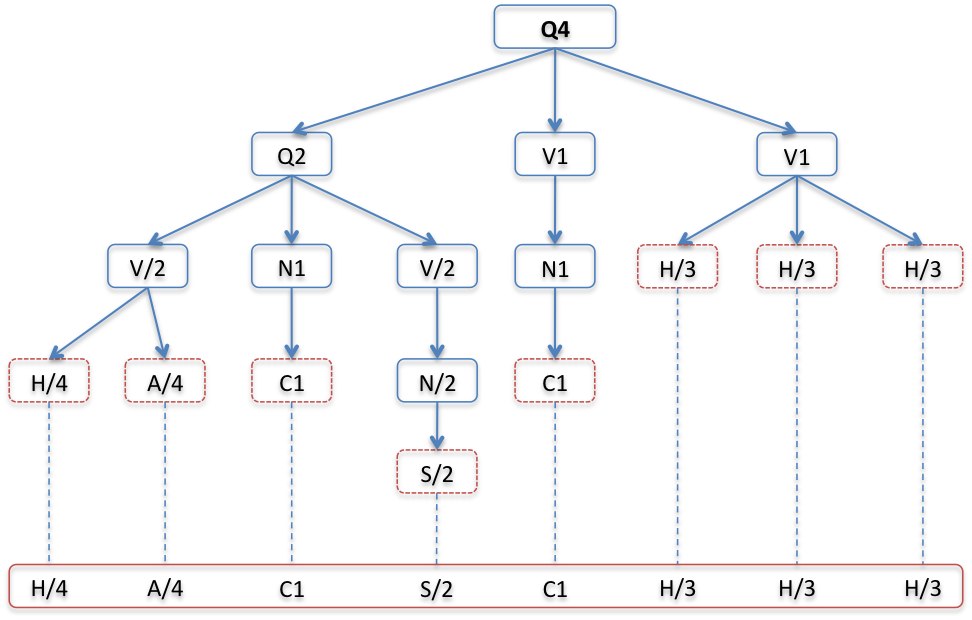
\includegraphics[scale=0.85]{figure/q4exampleparsetree.png}
  \captionof{figure}{Parse tree for the terminal sequence}
  \label{fig:q4exampleparsetree}
\end{figure}

Initially it would seem that if we were to adjust every rule then it would be mean our grammar weighting changes very easily. However if are increasing the weighting of a rule, we are essentially also decreasing the weighting of the the rules with the same variable. Adjusting many of the rules means we get a balanced weighting at the end. However this simple method is still not ideal as it would update/increasing the weighting of each rule by the same amount.

Ideally we'd want to be able to see after a batch run whether some rules have been selected more often than other rules. As a result we don't want to change all the rules, but only the ones that have been selected enough to strongly infer that they are responsible for generating the rhythmic aspect of the bars that were selected. In addition as our grammar is represented in a hierarchical tree structure, the leaves (N-rules) are likely to occur many times in a parse tree, compared to rules higher up the tree (Q or V rules). For example N1 $\rightarrow$ C1 is likely to come up more than once in a parse tree compared to a V rule, such as V1$\rightarrow$ H/3 H/3 H/3 (as seen in \ref{fig:q4exampleparsetree}). We also only get one Q4 and Q2 rule for each parse tree. 

A possible solution is to compare rules on the same level in the grammar hierarchy with each other. I.e. only compare N-rules against each other and update the rule which has a majority of selections. We can also make the adjusted amount a function of the current weighting and the number of times appeared per selected bar.

A possible function for a rule update for rule $r$ would be:

\[w' = w + \gamma N_r/N_{bars}\]


where $w'$ is the new weighting, $w$ is the original weighting and $N_r$ is the number of times the rule was selected in the process and $N_{bars}$ is the number of bars selected overall in the process. Gamma ($\gamma$) is a simple 'discount' factor (\textless  1) such as 0.1.

\section{Effectiveness of the Approach \& Criticisms}
One main criticism that we need to point out is that of course musical preferences will differ between users and thus it is unknown what the outcome will be like if we were to use different users as the fitness function to update the same grammar. However if we only used one person to act as the fitness function then we would end up with a grammar that produces output that sounds better for that one person, thus not generalising the solution. Though this can be argued to be either a good or bad aspect.

By now we recognise that due to the form of our output, it may be difficult to tell (or hear) whether this approach works or not. In addition we do not expect to see an immediate change to the output, mainly due to the number of examples that need to be evaluated before any significant change to the grammar weightings occur. The evaluation process can be quite lengthy as the listener must provide feedback for every piece of music, which in turn depends on the length of each piece. In addition the listener is likely to need to listen to the same piece a few times to make a confident judgement. Furthermore, we don't envision the user wanting to sit sit there all day evaluating pieces of music.

However we are confident that if the fitness function (the user) is well defined (in the sense that the user is able to give feedback on which bars they preferred, with an emphasis on rhythmic qualities) then over time there is no reason to not conclude that the updated grammar will generate more pleasing sounding melodies, and melodies which are more consistently pleasing to hear.


\chapter{Implementation}

\section{Overview}
The implementation of the blues improvisation using the grammar specified above is done in Java. Development itself was done using Eclipse IDE and it's tools which provides good support including refactoring tools and auto-completion. Build management of the project is handled by Apache Maven, which manages dependencies and plugins required for the project. ANTLR, a parser and lexer generator was used to parse the abstract tones grammar which will be explained further.

\section{Software Engineering Practices}
Software development is very much an iterative and incremental process. It is difficult to design the system correct on the first try and thus a lot of refactoring and changes may need to be done during the development process. In addition we hope that this piece of software forms a basis and platform upon which additional features can be implemented on top of. With both of these things in mind, it is important to make the system flexible and easy to extend. 

\subsection{Package Dependency/Management}
The program has been developed with software engineering considerations in mind. Classes are placed into appropriate packages such that packages do not have circular dependencies. [Show package dependency diagram?]. Interfaces are used to invert dependencies between packages and therefore reduce coupling in the system. 

\subsection{Extendability}
One of the aims of this project is that by making the program extendable, someone else can use the program as a foundation or basis for either exploring/implementing additional features or extending current features (such as a more comprehensive chord-scale system). As we shall see in the next section, by separating out the code to represent musical objects (things in the musical domain) we have built a library that can be used to represent and manipulate music with.

\section{Representation of Musical Objects}

\subsection{ABCJavaMusic}
In order to make manipulating musical notes easier, we decided to write a separate library (ABCJavaMusic) which allows us to represent musical notes/objects as java objects and represent/output them as ABC notation (see section \ref{abcnotation}). We could have used existing libraries and tools to convert from our abstract grammar to a musical score such as abc4j\footnote{http://code.google.com/p/abc4j/}. abc4j provides a parser that parses abc music files and in addition many features such as midi playback and music score display. Whilst these are useful things, other external tools can be used to achieve this often with better results, such as Ernie\footnote{http://geophysics.kos.net/ernie/} on Mac OSX (which can do midi playback and musical score display).

However the thing we are concerned with is the musical model. The musical model allows us to manipulate notes which is important as our computer essentially acts as the creative brain for generating notes. abc4j's musical model is very verbose and very similar to how abc notation itself represents music. 
ABCJavaMusic on the other hand represents music using a hierarchical structure as follows:

\begin{verbatim}
Full Score Line
  ->Treble/Bass Clef Score Line
    ->Bar
      ->Phrase
        ->Timed - Note Component (with duration)
          ->Note Component (with octave and accidental)
            ->Basic Note (with accidental)
\end{verbatim}

Having a hierarchical structure is useful as sometimes we may want information about a phrase, or about an individual note component. It is therefore beneficial overall to create a small/light-weight set of classes which do exactly what we want. This way, users can use this library to manipulate the musical objects for purposes similar to this project. Currently the objects can only print out as ABC notation.

\subsubsection{Example}
Here we demonstrate how we would represent some simple notes as Java objects. In Figure \ref{fig:abcnotationexample}, if we want to represent the notes as ABC notation (disregarding headers and bar lines in the ABC file) then it would look like:

\begin{verbatim}
C _D ^F3/2 _B,/2
\end{verbatim}

Where '$\_$' represents a flat, '$\wedge$' represents a sharp, and the ',' represents a lower octave (an apostrophe ['] represents a higher octave). The duration of the note (in this case in quarter/crotchet beats) is the number directly after the pitch of the note (C, D, E all have a duration of 1 quarter beat). So F\# and B both have /2 which indicates the duration is half of a quarter/crotchet beat, i.e. an eighth/quaver.

In Java, we would represent these notes by writing this code:

\begin{lstlisting}
MainNoteComponent middleCNote = 
      new MainNoteComponent(BasicNote.C);
TimedComponent middleCNoteQuarter = 
      new TimedComponent(middleCNote, Duration.quarter);

MainNoteComponent DFlatNote = 
      new MainNoteComponent(BasicNote.D, AccidentalShift.Flat);
TimedComponent DFlatNoteQuarter = 
      new TimedComponent(DFlatAboveMiddleCNote, Duration.quarter);

MainNoteComponent FSharpNote = 
      new MainNoteComponent(BasicNote.F, AccidentalShift.Sharp);
TimedComponent FSharpNoteDottedQuarter = 
      new TimedComponent(FSharpNote, Duration.dottedQuarter);

MainNoteComponent BFlatBelowMiddleCNote = 
      new MainNoteComponent(BasicNote.B, AccidentalShift.Flat, -1);
TimedComponent BFlatBelowMiddleCNoteEighth = 
      new TimedComponent(BFlatBelowMiddleCNote, Duration.eighth);

\end{lstlisting}

To represent a bar with those notes (all in one phrase), we would write:

\begin{lstlisting}
Bar bar = new Bar();
StandardTimedComponentPhrase phrase = 
      new StandardTimedComponentPhrase();
phrase.addtoComponentList(middleCNoteQuarter);
phrase.addtoComponentList(DFlatNoteQuarter);
phrase.addtoComponentList(FSharpNoteDottedQuarter);
phrase.addtoComponentList(BFlatBelowMiddleCNoteEighth);
bar.addToBar(phrase);

\end{lstlisting}

By calling bar.getAbcRepresentation() we would get the abc representation of these notes as seen above. The representation is very verbose, however it is not intended to be used to represent complete pieces of music. ABC notation is designed for the actual music representation. For example in our system, we use the library to convert the terminal sequence from our grammar (sequences of Tones) to actual musical notes, using heuristics / probabilistic methods. 

In addition if we wanted to get a full score line then we could do the following:

\begin{lstlisting}
TrebleClefScoreLine trebleClefScore = new TrebleClefScoreLine();
trebleClefScore.addBarToScoreLine(bar);
//we don't have anything in the bass clef, 
//so we just use a default empty bass clef score line
CombinedScoreLine fullScore = 
	new CombinedScoreLine(trebleClefScore, 
			      BassClefScoreLine.emptyScore());

\end{lstlisting}

\begin{figure}[here]
  \centering
  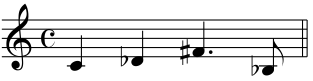
\includegraphics[scale=0.6]{figure/abcnotationexample.png}
  \captionof{figure}{Notes C, Dflat, Fsharp and Bflat}
  \label{fig:abcnotationexample}
\end{figure}

\subsubsection{Other useful things}
The library allows manipulation of notes, for example we can get a chromatic up or down note (one semitone apart) which is useful for approach tones, and in addition we can compare if notes are higher or lower than each other (frequency wise and on the keyboard). The hierarchical structure allows easy extension of the library if needed and provides a clear and logical way to work with musical objects in Java.

\subsection{ABC Notation} \label{abcnotation}
ABC notation is a text-based music notation system which allows simple representation of musical scores. It is widely used in folk and traditional music and is ASCII based. There is support for the format including tools to convert abc notation to midi and to printable scores (as pdf's). More about the notation can be read on the website \url{abcnotation.com}.

\section{Grammar Implementation}
In order to allow our program to be able to take in different grammars, (as long as the grammar follows the same naming conventions found in Keller's grammar), it would be ideal to be able to parse such grammars. A simple line-oriented parser will be enough to parse a grammar file which is specified line by line. ANTLR was chosen to do this as it integrates well with Java and has maven plugins will can manage the compilation of grammars into parser and lexer classes for Java. ANTLR's main use is for generating a recogniser for a language define by the context-free grammar which checks the syntax of the input (a sample program in the specified language). ANTLR also has a maven plugin which can manage compilation of grammars. The grammar for the musical grammar contains both parser and lexer rules and is to be specified using Extended Backus Naur Form with Regex expressions. 

\begin{verbatim}

grammar = {var '->' prodRule};
  
productionRule = vars '[' probability ']';

vars = '(' (var)+ ')' | var

var = (alpha)+ (digit)+ | (alpha)+ (digit)* '/' (digit)+;
probability = (digit)+ '.' (digit)+ | digit;
whitespace = [ \t\r\n]+

alpha = ('a'..'z' | 'A'..'Z');
digit = '0'..'9';

\end{verbatim}




\chapter{Evaluation}

\section{Overview}
Evaluation of a project in the domain of Computational Creativity is difficult. Assessment of such artistic output is very subjective, perhaps more so in other areas such as visual art generators or poetry generators. Music itself has however some more rigorous rules that determine at a basic level what sounds good or not. Human ears are all tuned similarly (i.e. we all hear the same things) and as such harmonics and frequencies play a significant role in the overall perception of the music. By implementing musical theory rules we can ensure that the music sounds 'correct' and stable at a basic level. Though in reality what is more important is that the music is interesting and intriguing to the listener. 
However the point of our program is not try to find a the 'correct' or optimal solution, but a solution that represents some form of a creative process.
There are two aspects of evaluation in Computational Creativity, one is evaluating/judging the output to determine whether the idea/concept is valuable or useful, and the other aspect is evaluating the creativity of the program itself, i.e. whether the program exhibits creativity. Here we evaluate this project using both aspects in order to be able to assess/measure the success and achievement of the project.

\section{Initial Evaluation of Program Aspects}
We start by doing some self evaluation on the strengths and weaknesses of the ideas and approaches that we have undertaken in project.

\subsection{Grammar}
The use of a grammar allowed us to produce melodies whilst constraining the rhythmic aspects of the music. The grammar given in Keller's paper \cite{keller07} is a good example of a grammar that works well in generating a large variety of music. A good grammar is able to produce music that is well structured all of the time and has interesting rhythmic qualities to it. The fact that the program takes in the grammar as an input means that users of the program can tweak and create their own grammars to generate different and unique music. However the down side of using a grammar that is an abstraction for musical notes is the difficulty in being able to produce a grammar that itself produces good melodies. In addition we mentioned previously that grammars have finite search spaces (in the case of our non recursive grammars) and thus music generation is limited per grammar.

\subsection{Rules - Musical Theory}
The idea of studying musical theory for this project was to be able to capture a subset of these rules into the program. These rules essentially tell the program what it can use to generate a melody, such as knowledge of the chord-scale system (which scales can be used on which chords) and also knowledge of avoid notes and dissonance. We have done this to some degree however it is not as comprehensive as we had hoped for. But from the simple model that we have currently, the generated music is able to sound interesting and unique whilst also sounding good musically.

\subsection{Heuristics}
We implemented some heuristics for choosing the musical notes given the terminal sequence from the grammar. The idea of a heuristic is to capture prior (human) experience without having to search the problem space for the 'optimal' solution. The heuristics, in particular the 'Better' heuristic is based on an approach which looks ahead to future chord tones as a point to 'resolve' the melody. The main concern with doing the 'Better' heuristic was to be able to implement the approach notes correctly (which the Simple heuristic could not do). Conversely, the rest of the 'Better' heuristic uses randomness and probabilities to choose notes. The randomness is an issue as it points to no real intent on the selection of the notes and as a result it can lead to some melodies not sounding as good as other melodies.

\section{External User Evaluation of Output}
The first aspect of CC evaluation is to determine from the output whether the idea/concept is valuable or useful. To do this we introduced an online survey which does a 'blind' test to compare music generated by our program and music generated by a human. Three pieces of music generated by the program were picked randomly out of a sample of 100 and two pieces were recorded by a human player (a jazz pianist). All pieces were the same length and used the same chord progression underneath (a ii-v-i-vi jazz standard) and users taking the survey do not know which piece is generated by which player.

Of course one thing to note is that our program is still limited in it's generation, for example the melody contains no chords and no ornaments (trills, crushed notes etc). In order to make the comparison fair, the human player was constrained to only play single notes in the melody. It is important to note however that a human player can still show a range of expression and creativity by playing only single notes. In addition both pieces were played through the same software instruments in the form of MIDI.

There are two main questions that we asked, the first of which is to try to identify which piece is generated by which player. This is similar to a turing test, in which we aim to test the program's ability to exhibit creative/intelligent behaviour that is equivalent to a human. The second question asks the users to rate each piece according to their preference on a Likert scale (using 5 degrees). This way we can compare the value or 'usefulness' of the generated pieces by seeing if the users enjoyed (or were intrigued by) listening to them.

From figure \ref{fig:identification}, the results showed that over the 23 participants, apart from Example 1, there was no real clear indication in terms of whether one piece was generated by a player or the computer. In addition most people guessed Example 3 wrong, however Example 3 was recorded using an extremely simplified playing style. Example 5 is more expressive and uses more Jazz elements (syncopation and some ornaments) however even though the majority of them guessed correctly, 43\% of them guessed it wrongly. With the computer generated examples we can see that the downside of using elements of randomness in the program can sometimes allow it to produce music that doesn't sound as creative or intelligent. However they can also produce fairly convincing pieces as evident in Examples 2 and 4.

From figure \ref{fig:opinion} we see that the results for the second questions are very much spread across the range. This is expected as this is of course a very subjective question. However this is a good indication that the computer generated pieces are interesting and intriguing in the respect that it procures a wide range of opinions. However the music itself is not as satisfying to listen to compared to the human compose Example 3 and 5 which have had some users choose the highest rating.  


\subsection{Issues \& Critique of Surveying}
One of the main issues is that our sample size is quite small (23). The number of results aren't enough to say that the results are statistically significant. On the other hand, the type of questions that the survey asks are quite subjective and thus it is not about the correct answer or the answer which is selected the most, but the fact that there is a spread of answers which means that in general, a decent amount of people cannot distinguish between one type or the other. 

There may be certain reasons why the human pieces were not clear to guess, one of them is that all pieces were recorded to MIDI, and quantised which gets rid of human expressions (such as slight imperfections and  sustain effects). This can make the identification harder and as those pieces don't seem as human. Similarly, a question was asked at the beginning of the survey asking users to categorise their musical theory knowledge from 'No music lessons taken' all the way to 'Good understanding of musical theory and Jazz theory'. The result was that most people had put down 'No music lessons taken' meaning that as naive listeners, their opinions would be mostly based on purely the aesthetic qualities of the music, rather than analysing the expressiveness and the complexity of jazz.

Additionally, even though this evaluation tells us that the music generated by the program is fairly convincing, it does directly try to answer the question of whether such output is creative or whether the process is creative. The next section explores this.


\begin{figure}[here]
  \centering
  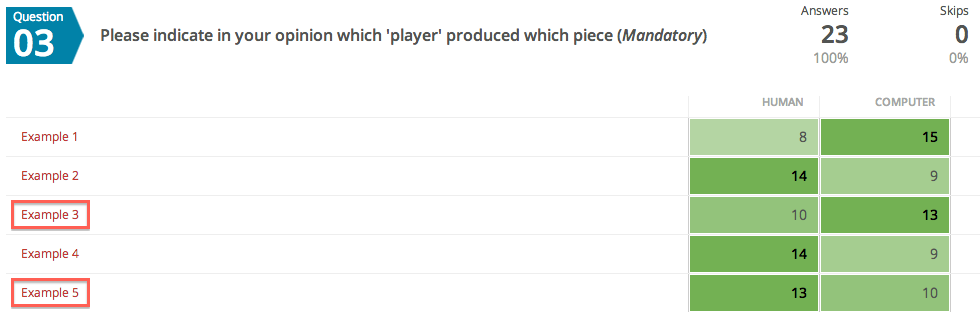
\includegraphics[scale=0.40]{figure/identification.png}
  \captionof{figure}{User Identification of Piece Generation, Example 3 and 5 (boxed) are composed by a human player}
  \label{fig:identification}
\end{figure}

\begin{figure}[here]
  \centering
  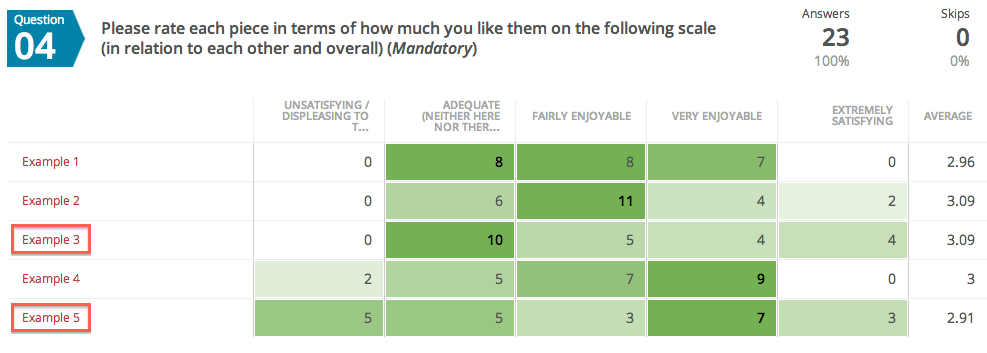
\includegraphics[scale=0.40]{figure/opinion.png}
  \captionof{figure}{User Opinion of Pieces, Example 3 and 5 (boxed) are composed by a human player}
  \label{fig:opinion}
\end{figure}

\section{Evaluating Creativeness in The Program}
Though the user evaluation approach (a kind of Turing test) can be used to infer creativity from the output. It is also useful to try and assess the creativity in the system itself. Though one could say that creativity in humans is usually judged by what they produce and so computers should be treated the same. In particular Ritchie argues this in his paper 'Some Empirical Criteria for Attributing Creativity to a Computer Program' in 2007 \cite{ritchie07}. The idea that the creativity is represented and evident in the output of the individual means that we should evaluate creativity based on the output alone and that evaluating the creativity in the system can be considered as circular.

In our case we assume that when human's take in artistic output such as the music produced by our program, their aesthetic opinions on the pieces are essentially a translation of the level of creativity that they perceive from the piece. The survey therefore gives us a 'judgement' of creativity, which is useful in one particular sense of creativity.

\subsection{The Creative Tripod}
But it is also useful to assess a more concrete idea of creativity. Simon Colton's 2008 paper \cite{colton08} argues that the creativity of the individual 'artist' is the primary consideration, with the output being the secondary. He gives an example using a scenario with visual art, where two canvasses with seemingly randomly placed dots look the same to the viewer, but one of them has a special meaning (some sort of meta-information such as a social network context) to the artist. Without the artist to tell them about the underlying meaning, the two pieces of art look the same and thus the creativity of both pieces would be measured equally, when in fact the processes behind creating them are very much different.

This leads us onto an assessment of creativity in systems using a Creative Tripod which was introduced by Simon Colton introduced in the same paper \cite{colton08}. A system that is creative must have the 3 attributes: skill, appreciation and imagination. 

A system is skillful if it is able to exhibit good knowledge of it's respective art form and can make decisions which leads to output which has the complexity which makes it seem skillful. Our program uses a rule based approach and so has knowledge of good rhythmic aspects (the abstract tones grammar) and also knowledge of how to pick appropriate notes to make a well formed piece of music. 

A system is appreciative if it can produce something of value and is able to take the best parts of it's work (given some feedback) and increase the value of it's output. User surveying and evaluation tells us that our program's output has value due to the range of opinions on the identification of the player and the aesthetic qualities of the pieces. In addition our reward-based learning extension allows our program to be appreciative by using a supervised learning approach which has our user act as a fitness function (i.e. the test input data in supervised learning terms) to provide feedback for generated pieces of music. However the extension is fairly simple/novel and only concentrates on updating the grammar weightings (rhythmic) aspects. But overall we can argue that our system shows some degree of appreciation. 

A system is imaginative if it produces work that sounds original and demonstrates independence from the creator (developer) and other composers/musicians. Our program does not rely on any existing pieces of music to come up with new pieces, generation of the melody is done using a heuristic which is essentially an abstracted idea of how to improvise melodies (using the creators experiences). However the melody depends on chord progressions which are supplied by the user and also the generation depends on a grammar which is also supplied by the user. However all this does is constrain what the program can generate (in a positive way). The heuristics on the other hand are implemented using fairly simple idea, using elements of randomness which we incorporate into a unique hash code / name for each individual piece. Overall we argue that our program is imaginative to some degree due to the originality of the work.

As such we have argued that our program satisfies the creative tripod's three attributes to some degree and so it can be said that the program is 'creative'. However we could say that the program does not exhibit these three attributes to a great degree, for example the program should be more appreciative be able to update and adapt a wider ranger of aspects in the program to improve and adapt it's output. In addition the current reward-based learning extension is untested due to the difficulties in evaluating the difference in output and also getting the grammar weightings to a point which makes a significant difference in the output.

\subsection{The FACE model}
The FACE model extends the creative tripod by allowing us to quantify creative processes by breaking the requirements/aspects of a creative act even further. We could then use this to compare against other systems that have also been evaluated using the FACE model, however in this case we use the FACE model to provide a formal description of the creative processes to accompany in the evaluation of our system. The model was recently introduced by Simon Colton in 2011\cite{coltonface2011}. In a similar and accompanying paper by Pease and Colton \cite{pease11}, the FACE model is seen as an alternative to the Turing test with which they argue has drawbacks such as encouraging pastiche (imitation) and penalising different styles of creativity. 

The name comes from the 4 aspects of the model, Framing, Aesthetics, Concepts and Expressions. For each of them are there two versions, a g-version which is the basic notion that the creativity is at a ground-level (i.e. simply generating a piece of music), and a p-version which is the notion that the creativity is at a process level, such that the system has a process for generating new ways to be creative. The following description of the 8 aspects of the FACE model is taken from the papers mentioned above:

\begin{description} [labelindent=0.6cm]  \itemsep0pt \parskip0pt \parsep0pt 
  \item[$F^{p}$] - a method for generating framing information
  \item[$F^{g}$] - an item of framing information
  \item[$A^{p}$] - a method for generating aesthetic measures 
  \item[$A^{g}$] - an aesthetic measure
  \item[$C^{p}$] - a method for generating concepts 
  \item[$C^{g}$] - a concept
  \item[$E^{p}$] - a method for generating expressions of a concept 
  \item[$E^{g}$] - an expression of a concept 
\end{description}

The model itself is stated not to be broad enough to cover every type of creative system out there, but is good enough as a starting guide for most systems. A systems creativity can then be expressed by a tuple which contains at exactly zero or one instance of each of the 4 aspects of FACE (have framing-p covers having framing-g for example, so there is no need for both). A more in depth explanation that comes directly from Colton's 2011 paper \cite{coltonface2011} tells us more about each aspect of FACE:

\begin{description} \itemsep1pt \parskip0pt \parsep0pt 
  \item[Framing Information ] - "a piece of natural language text that is comprehensible by people. Such framing information may be domain- specific, and adds value to the generative acts."
  \item[Aesthetic Measure] - "a function which takes as input a (concept, expression) pair – one of which can possibly be null – and outputs a real value be- tween 0 and infinity."
  \item[Concept] - "an executable program (or something which can be interpreted as such), which is ca- pable of taking input and producing output."
  \item[Expression of a Concept] - "an instance of an (input, output) pair produced when the concept’s program is executed."
\end{description}

From the definition of the p-version we can see that our program does not use any p-versions of FACE, partly due to the static nature of the rule based approach but mostly due to the complexity involved in having a creative-p process. So instead we try and analyse whether our program uses any of the g-versions, starting with the concept:

\begin{description}  \itemsep1pt \parskip0pt \parsep0pt 
  \item[Concept-g] - our program produces jazz compositions in an improvisational style using a rule based approach such as a grammar for rhythmic aspects and heuristics for pitch aspects. The idea of being able to use this natural-language based approach to generate convincing melodies is the concept in the FACE model. Therefore we say our program represents $C^{g}$.
  \item[Expression-g] - our program is expressive as it's main purpose is to produce output. The expression of the concept formally are the grammar rules and the underlying progression taken in as the input and the piece of music produced as the output. Therefore we say our program represents $E^{g}$. Though we have a reward based learning extension that changes the grammar weightings, it does not satisfy $E^{p}$ as this relies on direct user feedback to do so and therefore humans become involved in the creative aspect.
  \item[Aesthetics-g] - Our program does not have any internal aesthetic measures, it only relies on the user to provide feedback on the piece in order to improve its output. Thus our program does not satisfy $A^{g}$.
  \item[Framing-g] - Our program names each piece with a unique ID, but it does not give us real information about the piece, i.e. it is not comprehensible by people and does not justify the creative act. Thus we do not have $F^{g}$.
\end{description}


Our program's creative acts can therefore be represented as the tuple $\langle${$C^{g}$, $E^{g}$}$\rangle$. 
Framing information can be hard to do for pieces of music, especially if if it requires to justify why it chose certain notes/chords. It is also difficult to provide meaninful justification as to why a player would pick out certain notes etc. It would be better to explain the higher level aspects such as the choice of chord, or the choice of scale to use to improvise on top of the chord. However due to the current simple nature of how the program uses musical theory, it is difficult to have framing information which provides justification on some of the higher level aspects of the music generation. In addition if we wanted to name our pieces or provide some commentary on it in natural language, we would need to do it in such a way that the framing information does not seem arbitrary or random. This could involve studying the relationship between music and emotions/moods to provide a name that reflects the 

Aesthetic measures are more difficult to do, the program would need to have an idea of what good music sounds like. However it needs to be pointed out that the program itself use ideas and rules that essentially captures the aesthetic qualities of music (such as playing the scale that goes well with the chord), but it is used to create the output and not to assess it. Both of these can be achieved as part of further work in order to expand the creative aspects of the program. 


\chapter{Conclusion}

\section{Overview \& Achievements}
Our high level aims were to be able to produce jazz pieces that were convincing to pass off as human compositions. We aimed to use a grammar and musical theory rules to produce a tool that had the potential to be able to generate a vast variety of pleasant sounding music (using different chord progressions). The output that our program generates was able to pass off as human composed pieces and in addition the aesthetic qualities of the pieces were rated mostly at and above an 'enjoyable' level. Evaluation through user surveying tells us that differentiating between the music that the program generated and music that was composed at a similar difficulty level by a human musician was not easy.
In addition we also aimed to write some a program that can be used a basis for building upon and adding features to. We wrote a useful set of classes that allows representation and more importantly manipulation of musical objects. We believe that we have mostly succeeded in being able to achieve our high level aim and that we have laid out good groundwork in the form of our program and it has the potential for future work to take place on.

In addition our aims from a research standpoint were to use a predominantly rule-based approach to try and see whether our system could be seen as creative. Evaluation of the creative acts of the program showed us that our program satisfies the ideas of creative concepts and expressions of concepts to an adequate level, but lacks the framing information and aesthetic measures that other creative systems contain. 


\section{Further Work}
There is a lot of potential for further work in this project, with the main aim to be able to produce better sounding melodies (evaluated from subjective user feedback) and to make our program exhibit more creativeness (evaluated using models such as Simon Colton's Creative Tripod and FACE model). Here we talk about the different aspects of our program and lay down some potential future work in these areas:

\subsection{Grammar}
We mentioned previously that the down side of using a grammar that is an abstraction for musical notes is the difficulty in being able to produce a grammar that itself produces good melodies. Though a reward-based learning option exists, the grammar itself needs to have the right sequences of terminals and hierarchically needs to work (i.e. when expanded out all possibilities need to be good). One way to get around this would be to infer such grammars from existing pieces of work. This is explored already by Keller, Gillick and Tang \cite{kellergillick09}. 

Alternatively, we could possibly provide our program with a set of basic rhythmic ideas which the program can then produce a grammar out of (by learning/drawing inspiration from existing pieces of music). This would make the program creative at the process-level and provides even more possibilities for music generation (giving us Expression-p, $E^{p}$).

\subsection{Rules - Musical Theory}
Currently the chord scale system is very simple with each chord having compatible scale. In reality there could be more than one scale per chord which would increase the variety and tonality of the music generated. This would involve studying the scales and modes more, in particular melodic minor harmony is tricky to understand and to implement.

\subsection{Heuristics}
The Better Heuristic uses a lot of randomness (probabilistic methods) for choosing individual notes. Future work could include using more complex methods that justifies why we pick these notes or we could use more advanced random processes such as markov chains as explained below.

\subsubsection{Markov Chains as a Solution}
Markov chains are mathematical models which refer to a sequence/chain of states that a process goes through. They are stochastic processes and as such state changes/transitions are represented using transition matrices which contain probabilities of transitioning to the next state given the current state. The probability of moving to the next state depends on only the current state and not on any previous events and states.
 
For example we may instead want to use Markov Chains to choose Chord notes. The states would be the Chord notes themselves (the pitch) and transitions go from one Chord note to another Chord note. We may do this as we may find that going from one specific Chord note to another Chord note more appealing. We can come up with our own transition matrix or perhaps generate a different one for each piece that we generate. However implementing such a Markov Chain for the Chord note transitions such that the outcome is noticeably different is out of the scope of this project.

For the Colour and Scale tones, instead of a random selection, we could also use Markov Chains to do note selection. As we would expect multiple Colour and Scale tones per Chord note, we could use a multiple order Markov Chain to introduce a semblance of phrasing, such that we get a sense of familiarity and identity for a piece. For example a second order Markov Chain means that 3 note phrases can be constructed. 


\bibliographystyle{plain}
\bibliography{refs}

\begin{appendices}

\chapter{Example Output}
Here we have some examples of full output, the first 2 (figures \ref{fig:output42} and \ref{fig:output47}) of which are based on a II-V-I-VI progression (II-V-I is a standard jazz progression) in C major. The third (figure \ref{fig:flymeprog1} is an example using the progression from a famous jazz standard 'Fly Me to the Moon'. 

\begin{figure}[here]
  \centering
  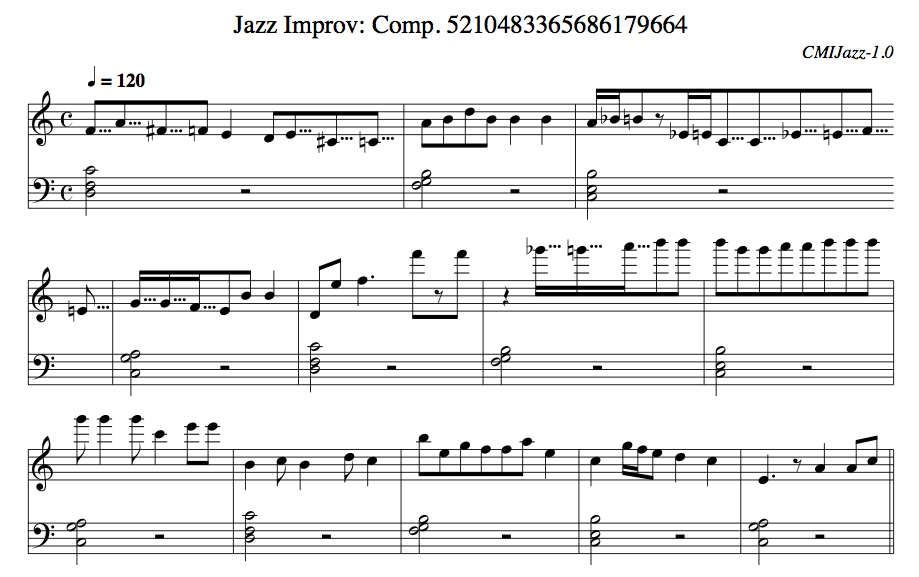
\includegraphics[scale=0.47]{figure/output42.png}
  \captionof{figure}{II-V-I Improvisation 1}
  \label{fig:output42}
\end{figure}

\begin{figure}[here]
  \centering
  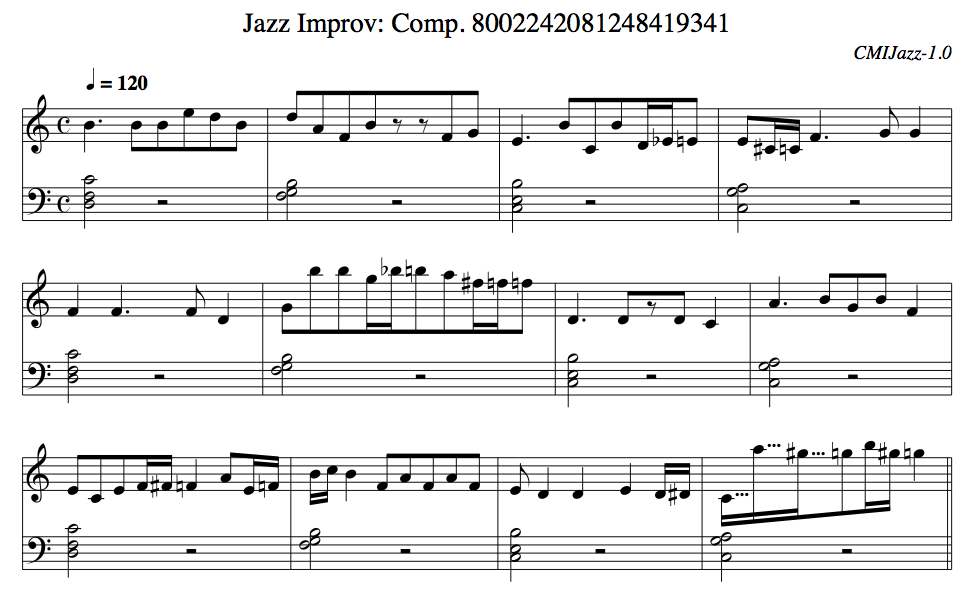
\includegraphics[scale=0.45]{figure/output47.png}
  \captionof{figure}{II-V-I Improvisation 2}
  \label{fig:output47}
\end{figure}

\begin{figure}[here]
  \centering
  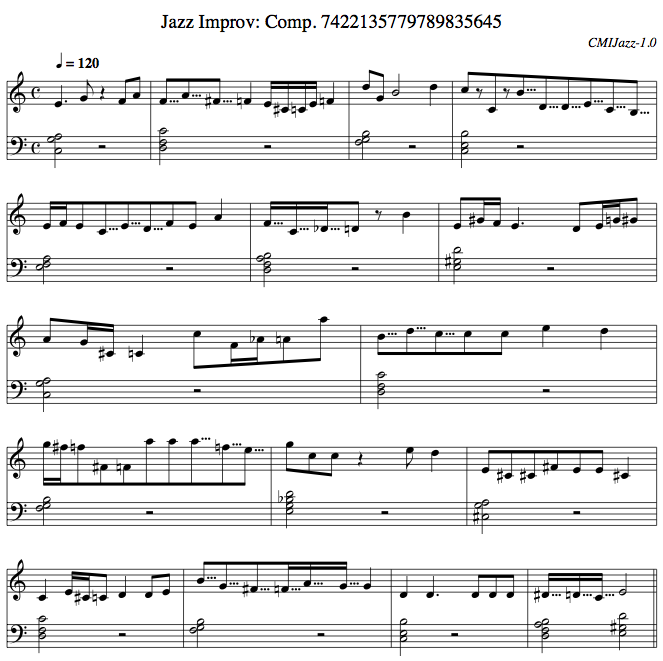
\includegraphics[scale=0.65]{figure/flymeprog1.png}
  \captionof{figure}{Improvisation using chord progression from Fly Me to the Moon}
  \label{fig:flymeprog1}
\end{figure}


\chapter{User Guide}
The program is a java application that at the moment can only be run through eclipse and the main method is located in the CMIBlues class. It takes up to 4 arguments (3 mandatory):

\begin{verbatim}
grammar_file   progression_file   option   number
\end{verbatim}

grammar_file and progression_file should be text files, bluesGrammar.txt an example grammar file and  progression1.txt, progression2.txt, progression3.txt are example progression files that are supplied.

`option' can either be `update' or `generate. `update' is used to update the grammar weightings by showing the user a number of pieces in which they have must give feedback on, if `number' is not supplied as the fourth argument then it defaults to showing just one example. If `generate' is selected then the program generates a number of pieces to abc files. Again if `number' is not specified then it defaults to one generated piece.


\end{appendices}

\end{document}


